\documentclass[]{article}
\usepackage{lmodern}
\usepackage{amssymb,amsmath}
\usepackage{ifxetex,ifluatex}
\usepackage{fixltx2e} % provides \textsubscript
\ifnum 0\ifxetex 1\fi\ifluatex 1\fi=0 % if pdftex
  \usepackage[T1]{fontenc}
  \usepackage[utf8]{inputenc}
\else % if luatex or xelatex
  \ifxetex
    \usepackage{mathspec}
  \else
    \usepackage{fontspec}
  \fi
  \defaultfontfeatures{Ligatures=TeX,Scale=MatchLowercase}
\fi
% use upquote if available, for straight quotes in verbatim environments
\IfFileExists{upquote.sty}{\usepackage{upquote}}{}
% use microtype if available
\IfFileExists{microtype.sty}{%
\usepackage{microtype}
\UseMicrotypeSet[protrusion]{basicmath} % disable protrusion for tt fonts
}{}
\usepackage[margin=1in]{geometry}
\usepackage{hyperref}
\hypersetup{unicode=true,
            pdftitle={Results.Rmd},
            pdfauthor={James Curran},
            pdfborder={0 0 0},
            breaklinks=true}
\urlstyle{same}  % don't use monospace font for urls
\usepackage{color}
\usepackage{fancyvrb}
\newcommand{\VerbBar}{|}
\newcommand{\VERB}{\Verb[commandchars=\\\{\}]}
\DefineVerbatimEnvironment{Highlighting}{Verbatim}{commandchars=\\\{\}}
% Add ',fontsize=\small' for more characters per line
\usepackage{framed}
\definecolor{shadecolor}{RGB}{248,248,248}
\newenvironment{Shaded}{\begin{snugshade}}{\end{snugshade}}
\newcommand{\AlertTok}[1]{\textcolor[rgb]{0.94,0.16,0.16}{#1}}
\newcommand{\AnnotationTok}[1]{\textcolor[rgb]{0.56,0.35,0.01}{\textbf{\textit{#1}}}}
\newcommand{\AttributeTok}[1]{\textcolor[rgb]{0.77,0.63,0.00}{#1}}
\newcommand{\BaseNTok}[1]{\textcolor[rgb]{0.00,0.00,0.81}{#1}}
\newcommand{\BuiltInTok}[1]{#1}
\newcommand{\CharTok}[1]{\textcolor[rgb]{0.31,0.60,0.02}{#1}}
\newcommand{\CommentTok}[1]{\textcolor[rgb]{0.56,0.35,0.01}{\textit{#1}}}
\newcommand{\CommentVarTok}[1]{\textcolor[rgb]{0.56,0.35,0.01}{\textbf{\textit{#1}}}}
\newcommand{\ConstantTok}[1]{\textcolor[rgb]{0.00,0.00,0.00}{#1}}
\newcommand{\ControlFlowTok}[1]{\textcolor[rgb]{0.13,0.29,0.53}{\textbf{#1}}}
\newcommand{\DataTypeTok}[1]{\textcolor[rgb]{0.13,0.29,0.53}{#1}}
\newcommand{\DecValTok}[1]{\textcolor[rgb]{0.00,0.00,0.81}{#1}}
\newcommand{\DocumentationTok}[1]{\textcolor[rgb]{0.56,0.35,0.01}{\textbf{\textit{#1}}}}
\newcommand{\ErrorTok}[1]{\textcolor[rgb]{0.64,0.00,0.00}{\textbf{#1}}}
\newcommand{\ExtensionTok}[1]{#1}
\newcommand{\FloatTok}[1]{\textcolor[rgb]{0.00,0.00,0.81}{#1}}
\newcommand{\FunctionTok}[1]{\textcolor[rgb]{0.00,0.00,0.00}{#1}}
\newcommand{\ImportTok}[1]{#1}
\newcommand{\InformationTok}[1]{\textcolor[rgb]{0.56,0.35,0.01}{\textbf{\textit{#1}}}}
\newcommand{\KeywordTok}[1]{\textcolor[rgb]{0.13,0.29,0.53}{\textbf{#1}}}
\newcommand{\NormalTok}[1]{#1}
\newcommand{\OperatorTok}[1]{\textcolor[rgb]{0.81,0.36,0.00}{\textbf{#1}}}
\newcommand{\OtherTok}[1]{\textcolor[rgb]{0.56,0.35,0.01}{#1}}
\newcommand{\PreprocessorTok}[1]{\textcolor[rgb]{0.56,0.35,0.01}{\textit{#1}}}
\newcommand{\RegionMarkerTok}[1]{#1}
\newcommand{\SpecialCharTok}[1]{\textcolor[rgb]{0.00,0.00,0.00}{#1}}
\newcommand{\SpecialStringTok}[1]{\textcolor[rgb]{0.31,0.60,0.02}{#1}}
\newcommand{\StringTok}[1]{\textcolor[rgb]{0.31,0.60,0.02}{#1}}
\newcommand{\VariableTok}[1]{\textcolor[rgb]{0.00,0.00,0.00}{#1}}
\newcommand{\VerbatimStringTok}[1]{\textcolor[rgb]{0.31,0.60,0.02}{#1}}
\newcommand{\WarningTok}[1]{\textcolor[rgb]{0.56,0.35,0.01}{\textbf{\textit{#1}}}}
\usepackage{graphicx,grffile}
\makeatletter
\def\maxwidth{\ifdim\Gin@nat@width>\linewidth\linewidth\else\Gin@nat@width\fi}
\def\maxheight{\ifdim\Gin@nat@height>\textheight\textheight\else\Gin@nat@height\fi}
\makeatother
% Scale images if necessary, so that they will not overflow the page
% margins by default, and it is still possible to overwrite the defaults
% using explicit options in \includegraphics[width, height, ...]{}
\setkeys{Gin}{width=\maxwidth,height=\maxheight,keepaspectratio}
\IfFileExists{parskip.sty}{%
\usepackage{parskip}
}{% else
\setlength{\parindent}{0pt}
\setlength{\parskip}{6pt plus 2pt minus 1pt}
}
\setlength{\emergencystretch}{3em}  % prevent overfull lines
\providecommand{\tightlist}{%
  \setlength{\itemsep}{0pt}\setlength{\parskip}{0pt}}
\setcounter{secnumdepth}{0}
% Redefines (sub)paragraphs to behave more like sections
\ifx\paragraph\undefined\else
\let\oldparagraph\paragraph
\renewcommand{\paragraph}[1]{\oldparagraph{#1}\mbox{}}
\fi
\ifx\subparagraph\undefined\else
\let\oldsubparagraph\subparagraph
\renewcommand{\subparagraph}[1]{\oldsubparagraph{#1}\mbox{}}
\fi

%%% Use protect on footnotes to avoid problems with footnotes in titles
\let\rmarkdownfootnote\footnote%
\def\footnote{\protect\rmarkdownfootnote}

%%% Change title format to be more compact
\usepackage{titling}

% Create subtitle command for use in maketitle
\providecommand{\subtitle}[1]{
  \posttitle{
    \begin{center}\large#1\end{center}
    }
}

\setlength{\droptitle}{-2em}

  \title{Results.Rmd}
    \pretitle{\vspace{\droptitle}\centering\huge}
  \posttitle{\par}
    \author{James Curran}
    \preauthor{\centering\large\emph}
  \postauthor{\par}
      \predate{\centering\large\emph}
  \postdate{\par}
    \date{28/06/2019}


\begin{document}
\maketitle

\hypertarget{model-g_0---no-effects}{%
\subsection{\texorpdfstring{Model \(g_0\) - no
effects}{Model g\_0 - no effects}}\label{model-g_0---no-effects}}

\begin{figure}
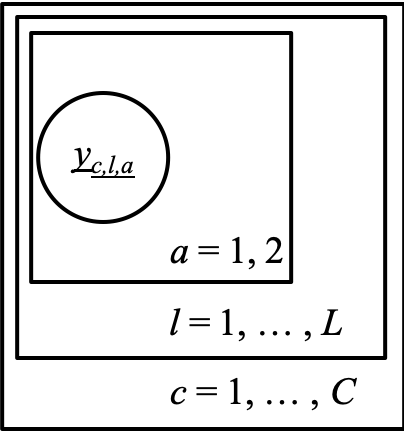
\includegraphics[width=0.25\linewidth]{g0} \caption{Model $g_0$}\label{fig:g0}
\end{figure}

\textbf{Model:} \[
y_{c,l,a} \sim \Gamma(r,s)
\] If \[
\mathrm{E}[y_{c,l,a}]) = \log(\mu)\mbox{ and }\mathrm{Var}[y_{c,l,a}] = \sigma^2
\] then we let \[
r  = \frac{\mu^2}{\sigma^2}\mbox{ and }s = \frac{\mu}{\sigma^2}
\] Our prior on \(\sigma^2\) is \(inverse-\Gamma(0.001, 0.001)\), and
our prior on \(\log(\mu)\) is \(N(0, 10^6)\).

First I will load up the results.

\begin{Shaded}
\begin{Highlighting}[]
\KeywordTok{library}\NormalTok{(here)}
\KeywordTok{load}\NormalTok{(}\StringTok{"../systematic/g-0.Rda"}\NormalTok{)}
\end{Highlighting}
\end{Shaded}

Given that we only have one chain, we might as well simultaneously pull
the results out of the list, and turn the results into a data frame.
This will make our code easier. \textbf{Note this type conversion won't
work unless rjags is loaded}

\begin{Shaded}
\begin{Highlighting}[]
\KeywordTok{library}\NormalTok{(rjags)}
\NormalTok{g0.df =}\StringTok{ }\KeywordTok{as.data.frame}\NormalTok{(}\KeywordTok{as.matrix}\NormalTok{(sim.sample))}
\end{Highlighting}
\end{Shaded}

I'll do this with ggplot2 so I can teach myself something

\begin{Shaded}
\begin{Highlighting}[]
\KeywordTok{library}\NormalTok{(ggplot2)}
\KeywordTok{library}\NormalTok{(tidyverse)}
\NormalTok{p =}\StringTok{ }\NormalTok{g0.df }\OperatorTok\StringTok{ }
\StringTok{  }\KeywordTok{ggplot}\NormalTok{(}\KeywordTok{aes}\NormalTok{(}\DataTypeTok{x =}\NormalTok{ tau)) }\OperatorTok{+}
\StringTok{  }\KeywordTok{geom_density}\NormalTok{()}
\NormalTok{p}
\end{Highlighting}
\end{Shaded}

\includegraphics{results_files/figure-latex/unnamed-chunk-3-1.pdf}

We want plots of shape and rate, so I will create them in the data frame
first as we didn't store them during the sampling

\begin{Shaded}
\begin{Highlighting}[]
\NormalTok{g0.df =}\StringTok{ }\NormalTok{g0.df }\OperatorTok\StringTok{ }
\StringTok{  }\KeywordTok{mutate}\NormalTok{(}\DataTypeTok{shape =} \KeywordTok{exp}\NormalTok{(log.Mu)}\OperatorTok{^}\DecValTok{2} \OperatorTok{*}\StringTok{ }\NormalTok{tau) }\OperatorTok\StringTok{ }
\StringTok{  }\KeywordTok{mutate}\NormalTok{(}\DataTypeTok{rate =} \KeywordTok{exp}\NormalTok{(log.Mu) }\OperatorTok{*}\StringTok{ }\NormalTok{tau)}
\end{Highlighting}
\end{Shaded}

\begin{Shaded}
\begin{Highlighting}[]
\NormalTok{p =}\StringTok{ }\NormalTok{g0.df }\OperatorTok\StringTok{ }
\StringTok{  }\KeywordTok{ggplot}\NormalTok{(}\KeywordTok{aes}\NormalTok{(}\DataTypeTok{x =}\NormalTok{ shape))}\OperatorTok{+}
\StringTok{  }\KeywordTok{geom_density}\NormalTok{()}
\NormalTok{p}
\end{Highlighting}
\end{Shaded}

\includegraphics{results_files/figure-latex/unnamed-chunk-5-1.pdf}

\begin{Shaded}
\begin{Highlighting}[]
\NormalTok{p =}\StringTok{ }\NormalTok{g0.df }\OperatorTok\StringTok{ }
\StringTok{  }\KeywordTok{ggplot}\NormalTok{(}\KeywordTok{aes}\NormalTok{(}\DataTypeTok{x =}\NormalTok{ rate))}\OperatorTok{+}
\StringTok{  }\KeywordTok{geom_density}\NormalTok{()}
\NormalTok{p}
\end{Highlighting}
\end{Shaded}

\includegraphics{results_files/figure-latex/unnamed-chunk-6-1.pdf}

\begin{Shaded}
\begin{Highlighting}[]
\KeywordTok{library}\NormalTok{(gNanoPkg)}
\NormalTok{gNano.df =}\StringTok{ }\KeywordTok{readData}\NormalTok{()}

\NormalTok{rateDensity =}\StringTok{ }\KeywordTok{density}\NormalTok{(g0.df}\OperatorTok{$}\NormalTok{rate)}
\NormalTok{shapeDensity =}\StringTok{ }\KeywordTok{density}\NormalTok{(g0.df}\OperatorTok{$}\NormalTok{shape)}

\NormalTok{rateMode =}\StringTok{ }\NormalTok{rateDensity}\OperatorTok{$}\NormalTok{x[}\KeywordTok{which.max}\NormalTok{(rateDensity}\OperatorTok{$}\NormalTok{y)]}
\NormalTok{shapeMode =}\StringTok{ }\NormalTok{shapeDensity}\OperatorTok{$}\NormalTok{x[}\KeywordTok{which.max}\NormalTok{(shapeDensity}\OperatorTok{$}\NormalTok{y)]}

\NormalTok{density.df =}\StringTok{ }\KeywordTok{data.frame}\NormalTok{(}\DataTypeTok{x =} \KeywordTok{seq}\NormalTok{(}\DecValTok{1}\NormalTok{, }\DecValTok{30000}\NormalTok{, }\DecValTok{1}\NormalTok{)) }\OperatorTok\StringTok{ }
\StringTok{  }\KeywordTok{mutate}\NormalTok{(}\DataTypeTok{y =} \KeywordTok{dgamma}\NormalTok{(x, }\DataTypeTok{rate =}\NormalTok{ rateMode, }\DataTypeTok{shape =}\NormalTok{ shapeMode))}

\NormalTok{p =}\StringTok{ }\NormalTok{gNano.df }\OperatorTok\StringTok{ }
\StringTok{  }\KeywordTok{ggplot}\NormalTok{(}\KeywordTok{aes}\NormalTok{(}\DataTypeTok{x =}\NormalTok{ obs, }\DataTypeTok{y =} \KeywordTok{stat}\NormalTok{(density))) }\OperatorTok{+}\StringTok{ }
\StringTok{  }\KeywordTok{geom_histogram}\NormalTok{(}\DataTypeTok{binwidth =} \DecValTok{400}\NormalTok{) }\OperatorTok{+}
\StringTok{  }\KeywordTok{geom_line}\NormalTok{(}\DataTypeTok{data =}\NormalTok{ density.df, }\KeywordTok{aes}\NormalTok{(x, y))}
\NormalTok{p}
\end{Highlighting}
\end{Shaded}

\includegraphics{results_files/figure-latex/unnamed-chunk-7-1.pdf}

Plot the observed vs the expected peak heights

\begin{Shaded}
\begin{Highlighting}[]
\NormalTok{expected =}\StringTok{ }\NormalTok{g0.df }\OperatorTok\StringTok{ }
\StringTok{  }\KeywordTok{select}\NormalTok{(}\KeywordTok{starts_with}\NormalTok{(}\StringTok{"pred"}\NormalTok{)) }\OperatorTok\StringTok{ }
\StringTok{  }\KeywordTok{summarise_all}\NormalTok{(mean) }\OperatorTok\StringTok{ }
\StringTok{  }\KeywordTok{unlist}\NormalTok{()}
  
\NormalTok{plot.df =}\StringTok{ }\KeywordTok{data.frame}\NormalTok{(}\DataTypeTok{observed =}\NormalTok{ gNano.df}\OperatorTok{$}\NormalTok{obs, }\DataTypeTok{expected =}\NormalTok{ expected)}
\NormalTok{p =}\StringTok{ }\NormalTok{plot.df }\OperatorTok\StringTok{ }
\StringTok{  }\KeywordTok{ggplot}\NormalTok{(}\KeywordTok{aes}\NormalTok{(}\DataTypeTok{x =} \KeywordTok{log10}\NormalTok{(observed), }\DataTypeTok{y =} \KeywordTok{log10}\NormalTok{(expected))) }\OperatorTok{+}
\StringTok{           }\KeywordTok{geom_point}\NormalTok{() }\OperatorTok{+}
\StringTok{           }\KeywordTok{geom_abline}\NormalTok{(}\KeywordTok{aes}\NormalTok{(}\DataTypeTok{intercept =} \DecValTok{0}\NormalTok{, }\DataTypeTok{slope =} \DecValTok{1}\NormalTok{)) }\OperatorTok{+}\StringTok{ }
\StringTok{          }\KeywordTok{xlim}\NormalTok{(}\DecValTok{2}\NormalTok{, }\DecValTok{5}\NormalTok{) }\OperatorTok{+}
\StringTok{          }\KeywordTok{ylim}\NormalTok{(}\DecValTok{2}\NormalTok{, }\DecValTok{5}\NormalTok{)}
\NormalTok{p}
\end{Highlighting}
\end{Shaded}

\begin{verbatim}
## Warning: Removed 8 rows containing missing values (geom_point).
\end{verbatim}

\includegraphics{results_files/figure-latex/unnamed-chunk-8-1.pdf}

\hypertarget{model-g_1---profile-effects}{%
\subsection{\texorpdfstring{Model \(g_1\) - profile
effects}{Model g\_1 - profile effects}}\label{model-g_1---profile-effects}}

\begin{figure}
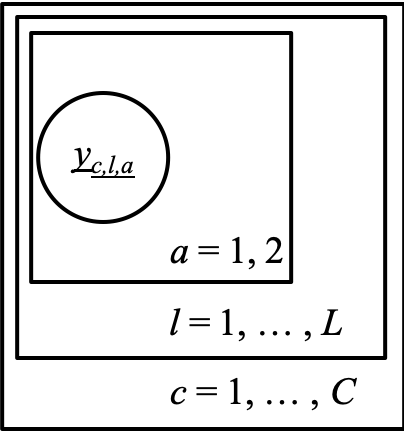
\includegraphics[width=0.25\linewidth]{g1} \caption{Model $g_1$}\label{fig:g1}
\end{figure}

Let's have a look at the profile effects. I like to use error bar plots

\begin{Shaded}
\begin{Highlighting}[]
\KeywordTok{load}\NormalTok{(}\StringTok{"../systematic/g-1.Rda"}\NormalTok{)}
\NormalTok{g1.df =}\StringTok{ }\KeywordTok{as.data.frame}\NormalTok{(}\KeywordTok{as.matrix}\NormalTok{(sim.sample))}
\end{Highlighting}
\end{Shaded}

This code is not elegant, and is probably stupid but then so is the
tidyverse a lot of the time :-)

\begin{Shaded}
\begin{Highlighting}[]
\NormalTok{lb =}\StringTok{ }\NormalTok{g1.df }\OperatorTok\StringTok{ }
\StringTok{    }\KeywordTok{select}\NormalTok{(}\KeywordTok{starts_with}\NormalTok{(}\StringTok{"beta.profile"}\NormalTok{)) }\OperatorTok\StringTok{ }
\StringTok{    }\KeywordTok{summarise_all}\NormalTok{(quantile, }\DataTypeTok{prob =} \KeywordTok{c}\NormalTok{(}\FloatTok{0.025}\NormalTok{)) }\OperatorTok\StringTok{ }
\StringTok{  }\KeywordTok{unlist}\NormalTok{()}

\NormalTok{med =}\StringTok{ }\NormalTok{g1.df }\OperatorTok\StringTok{ }
\StringTok{  }\KeywordTok{select}\NormalTok{(}\KeywordTok{starts_with}\NormalTok{(}\StringTok{"beta.profile"}\NormalTok{)) }\OperatorTok\StringTok{ }
\StringTok{  }\KeywordTok{summarise_all}\NormalTok{(quantile, }\DataTypeTok{prob =} \KeywordTok{c}\NormalTok{(}\FloatTok{0.5}\NormalTok{)) }\OperatorTok\StringTok{ }
\StringTok{  }\KeywordTok{unlist}\NormalTok{()}

\NormalTok{ub =}\StringTok{ }\NormalTok{g1.df }\OperatorTok\StringTok{ }
\StringTok{  }\KeywordTok{select}\NormalTok{(}\KeywordTok{starts_with}\NormalTok{(}\StringTok{"beta.profile"}\NormalTok{)) }\OperatorTok\StringTok{ }
\StringTok{  }\KeywordTok{summarise_all}\NormalTok{(quantile, }\DataTypeTok{prob =} \KeywordTok{c}\NormalTok{(}\FloatTok{0.975}\NormalTok{)) }\OperatorTok\StringTok{ }
\StringTok{  }\KeywordTok{unlist}\NormalTok{()}

\NormalTok{quantiles.df =}\StringTok{ }\KeywordTok{data.frame}\NormalTok{(}\DataTypeTok{lb =}\NormalTok{ lb, }\DataTypeTok{med =}\NormalTok{ med, }\DataTypeTok{ub =}\NormalTok{ ub) }\OperatorTok\StringTok{ }
\StringTok{  }\KeywordTok{mutate}\NormalTok{(}\DataTypeTok{profile =} \DecValTok{1}\OperatorTok{:}\DecValTok{102}\NormalTok{)}

\NormalTok{p =}\StringTok{ }\KeywordTok{ggplot}\NormalTok{(}\DataTypeTok{data =}\NormalTok{ quantiles.df, }\KeywordTok{aes}\NormalTok{(}\DataTypeTok{x =}\NormalTok{ profile, }\DataTypeTok{y =}\NormalTok{ quantiles.df}\OperatorTok{$}\NormalTok{med)) }\OperatorTok{+}
\StringTok{  }\KeywordTok{geom_point}\NormalTok{(}\KeywordTok{aes}\NormalTok{(}\DataTypeTok{col =} \StringTok{"red"}\NormalTok{), }\DataTypeTok{show.legend =} \OtherTok{FALSE}\NormalTok{) }\OperatorTok{+}\StringTok{ }
\StringTok{  }\KeywordTok{geom_errorbar}\NormalTok{(}\KeywordTok{aes}\NormalTok{(}\DataTypeTok{ymin =}\NormalTok{ lb, }\DataTypeTok{ymax =}\NormalTok{ ub)) }\OperatorTok{+}
\StringTok{  }\KeywordTok{geom_hline}\NormalTok{(}\KeywordTok{aes}\NormalTok{(}\DataTypeTok{yintercept=}\DecValTok{0}\NormalTok{)) }\OperatorTok{+}
\StringTok{  }\KeywordTok{ylab}\NormalTok{(}\KeywordTok{bquote}\NormalTok{(beta[Profile])) }\OperatorTok{+}\StringTok{ }
\StringTok{  }\KeywordTok{xlab}\NormalTok{(}\StringTok{"Profile"}\NormalTok{)}
  
\NormalTok{p}
\end{Highlighting}
\end{Shaded}

\includegraphics{results_files/figure-latex/unnamed-chunk-10-1.pdf}

\begin{Shaded}
\begin{Highlighting}[]
\NormalTok{aph =}\StringTok{ }\NormalTok{gNano.df }\OperatorTok\StringTok{ }
\StringTok{  }\KeywordTok{group_by}\NormalTok{(prof) }\OperatorTok\StringTok{ }
\StringTok{  }\KeywordTok{summarise}\NormalTok{(}\DataTypeTok{aph =} \KeywordTok{mean}\NormalTok{(}\KeywordTok{log}\NormalTok{(obs), }\DataTypeTok{na.rm =} \OtherTok{TRUE}\NormalTok{)) }\OperatorTok\StringTok{ }
\StringTok{  }\KeywordTok{pull}\NormalTok{(aph)}


\NormalTok{meanEffect =}\StringTok{ }\NormalTok{g1.df }\OperatorTok\StringTok{ }
\StringTok{  }\KeywordTok{select}\NormalTok{(}\KeywordTok{starts_with}\NormalTok{(}\StringTok{"beta.profile"}\NormalTok{)) }\OperatorTok\StringTok{ }
\StringTok{  }\KeywordTok{summarise_all}\NormalTok{(mean, }\DataTypeTok{na.rm =} \OtherTok{TRUE}\NormalTok{) }\OperatorTok\StringTok{ }
\StringTok{  }\KeywordTok{unlist}\NormalTok{()}
  
\NormalTok{plot.df =}\StringTok{ }\KeywordTok{data.frame}\NormalTok{(}\DataTypeTok{aph =}\NormalTok{ aph, }\DataTypeTok{meanEffect =}\NormalTok{ meanEffect)}
\NormalTok{p =}\StringTok{ }\NormalTok{plot.df }\OperatorTok\StringTok{ }
\StringTok{  }\KeywordTok{ggplot}\NormalTok{(}\KeywordTok{aes}\NormalTok{(}\DataTypeTok{x =}\NormalTok{ aph, }\DataTypeTok{y =}\NormalTok{ meanEffect)) }\OperatorTok{+}\StringTok{ }
\StringTok{  }\KeywordTok{geom_point}\NormalTok{(}\DataTypeTok{show.legend =} \OtherTok{FALSE}\NormalTok{) }\OperatorTok{+}
\StringTok{  }\KeywordTok{geom_smooth}\NormalTok{()}

\NormalTok{p}
\end{Highlighting}
\end{Shaded}

\includegraphics{results_files/figure-latex/unnamed-chunk-11-1.pdf}

Plot the observed vs the expected peak heights

\begin{Shaded}
\begin{Highlighting}[]
\NormalTok{expected =}\StringTok{ }\NormalTok{g1.df }\OperatorTok\StringTok{ }
\StringTok{  }\KeywordTok{select}\NormalTok{(}\KeywordTok{starts_with}\NormalTok{(}\StringTok{"pred"}\NormalTok{)) }\OperatorTok\StringTok{ }
\StringTok{  }\KeywordTok{summarise_all}\NormalTok{(mean) }\OperatorTok\StringTok{ }
\StringTok{  }\KeywordTok{unlist}\NormalTok{()}
  
\NormalTok{plot.df =}\StringTok{ }\KeywordTok{data.frame}\NormalTok{(}\DataTypeTok{observed =}\NormalTok{ gNano.df}\OperatorTok{$}\NormalTok{obs, }\DataTypeTok{expected =}\NormalTok{ expected)}
\NormalTok{p =}\StringTok{ }\NormalTok{plot.df }\OperatorTok\StringTok{ }
\StringTok{  }\KeywordTok{ggplot}\NormalTok{(}\KeywordTok{aes}\NormalTok{(}\DataTypeTok{x =} \KeywordTok{log10}\NormalTok{(observed), }\DataTypeTok{y =} \KeywordTok{log10}\NormalTok{(expected))) }\OperatorTok{+}
\StringTok{           }\KeywordTok{geom_point}\NormalTok{() }\OperatorTok{+}
\StringTok{           }\KeywordTok{geom_abline}\NormalTok{(}\KeywordTok{aes}\NormalTok{(}\DataTypeTok{intercept =} \DecValTok{0}\NormalTok{, }\DataTypeTok{slope =} \DecValTok{1}\NormalTok{)) }\OperatorTok{+}\StringTok{ }
\StringTok{          }\KeywordTok{xlim}\NormalTok{(}\DecValTok{2}\NormalTok{, }\DecValTok{5}\NormalTok{) }\OperatorTok{+}
\StringTok{          }\KeywordTok{ylim}\NormalTok{(}\DecValTok{2}\NormalTok{, }\DecValTok{5}\NormalTok{)}
\NormalTok{p}
\end{Highlighting}
\end{Shaded}

\begin{verbatim}
## Warning: Removed 8 rows containing missing values (geom_point).
\end{verbatim}

\includegraphics{results_files/figure-latex/unnamed-chunk-12-1.pdf}

\hypertarget{model-g_2---locus-effects}{%
\subsection{\texorpdfstring{Model \(g_2\) - locus
effects}{Model g\_2 - locus effects}}\label{model-g_2---locus-effects}}

\begin{figure}
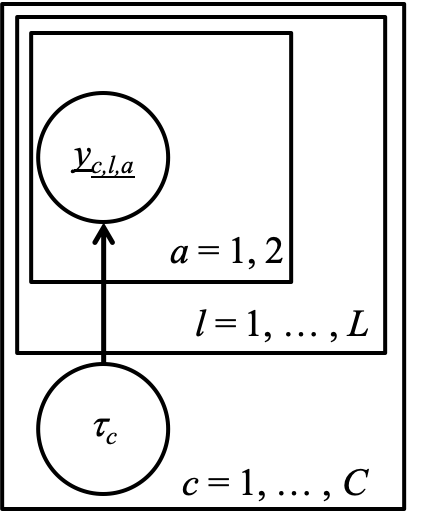
\includegraphics[width=0.25\linewidth]{g2} \caption{Model $g_2$}\label{fig:g2}
\end{figure}

\begin{Shaded}
\begin{Highlighting}[]
\KeywordTok{load}\NormalTok{(}\StringTok{"../systematic/g-2.Rda"}\NormalTok{)}
\NormalTok{g2.df =}\StringTok{ }\KeywordTok{data.frame}\NormalTok{(}\KeywordTok{as.matrix}\NormalTok{(sim.sample[[}\DecValTok{1}\NormalTok{]]))}

\NormalTok{lb =}\StringTok{ }\NormalTok{g2.df }\OperatorTok\StringTok{ }
\StringTok{    }\KeywordTok{select}\NormalTok{(}\KeywordTok{starts_with}\NormalTok{(}\StringTok{"alpha.locus"}\NormalTok{)) }\OperatorTok\StringTok{ }
\StringTok{    }\KeywordTok{summarise_all}\NormalTok{(quantile, }\DataTypeTok{prob =} \KeywordTok{c}\NormalTok{(}\FloatTok{0.025}\NormalTok{)) }\OperatorTok\StringTok{ }
\StringTok{  }\KeywordTok{unlist}\NormalTok{()}

\NormalTok{med =}\StringTok{ }\NormalTok{g2.df }\OperatorTok\StringTok{ }
\StringTok{  }\KeywordTok{select}\NormalTok{(}\KeywordTok{starts_with}\NormalTok{(}\StringTok{"alpha.locus"}\NormalTok{)) }\OperatorTok\StringTok{ }
\StringTok{  }\KeywordTok{summarise_all}\NormalTok{(quantile, }\DataTypeTok{prob =} \KeywordTok{c}\NormalTok{(}\FloatTok{0.5}\NormalTok{)) }\OperatorTok\StringTok{ }
\StringTok{  }\KeywordTok{unlist}\NormalTok{()}

\NormalTok{ub =}\StringTok{ }\NormalTok{g2.df }\OperatorTok\StringTok{ }
\StringTok{  }\KeywordTok{select}\NormalTok{(}\KeywordTok{starts_with}\NormalTok{(}\StringTok{"alpha.locus"}\NormalTok{)) }\OperatorTok\StringTok{ }
\StringTok{  }\KeywordTok{summarise_all}\NormalTok{(quantile, }\DataTypeTok{prob =} \KeywordTok{c}\NormalTok{(}\FloatTok{0.975}\NormalTok{)) }\OperatorTok\StringTok{ }
\StringTok{  }\KeywordTok{unlist}\NormalTok{()}

\NormalTok{quantiles.df =}\StringTok{ }\KeywordTok{data.frame}\NormalTok{(}\DataTypeTok{lb =}\NormalTok{ lb, }\DataTypeTok{med =}\NormalTok{ med, }\DataTypeTok{ub =}\NormalTok{ ub) }\OperatorTok\StringTok{ }
\StringTok{  }\KeywordTok{mutate}\NormalTok{(}\DataTypeTok{locus =} \DecValTok{1}\OperatorTok{:}\DecValTok{31}\NormalTok{)}

\NormalTok{p =}\StringTok{ }\KeywordTok{ggplot}\NormalTok{(}\DataTypeTok{data =}\NormalTok{ quantiles.df, }\KeywordTok{aes}\NormalTok{(}\DataTypeTok{x =}\NormalTok{ locus, }\DataTypeTok{y =}\NormalTok{ quantiles.df}\OperatorTok{$}\NormalTok{med)) }\OperatorTok{+}
\StringTok{  }\KeywordTok{geom_point}\NormalTok{(}\KeywordTok{aes}\NormalTok{(}\DataTypeTok{col =} \StringTok{"red"}\NormalTok{), }\DataTypeTok{show.legend =} \OtherTok{FALSE}\NormalTok{) }\OperatorTok{+}\StringTok{ }
\StringTok{  }\KeywordTok{geom_errorbar}\NormalTok{(}\KeywordTok{aes}\NormalTok{(}\DataTypeTok{ymin =}\NormalTok{ lb, }\DataTypeTok{ymax =}\NormalTok{ ub)) }\OperatorTok{+}
\StringTok{  }\KeywordTok{geom_hline}\NormalTok{(}\KeywordTok{aes}\NormalTok{(}\DataTypeTok{yintercept=}\DecValTok{0}\NormalTok{)) }\OperatorTok{+}
\StringTok{  }\KeywordTok{ylab}\NormalTok{(}\KeywordTok{bquote}\NormalTok{(alpha[locus])) }\OperatorTok{+}\StringTok{ }
\StringTok{  }\KeywordTok{xlab}\NormalTok{(}\StringTok{"Locus"}\NormalTok{)}
  
\NormalTok{p}
\end{Highlighting}
\end{Shaded}

\includegraphics{results_files/figure-latex/unnamed-chunk-13-1.pdf}

Plot the observed vs the expected peak heights

\begin{Shaded}
\begin{Highlighting}[]
\NormalTok{expected =}\StringTok{ }\NormalTok{g2.df }\OperatorTok\StringTok{ }
\StringTok{  }\KeywordTok{select}\NormalTok{(}\KeywordTok{starts_with}\NormalTok{(}\StringTok{"pred"}\NormalTok{)) }\OperatorTok\StringTok{ }
\StringTok{  }\KeywordTok{summarise_all}\NormalTok{(mean) }\OperatorTok\StringTok{ }
\StringTok{  }\KeywordTok{unlist}\NormalTok{()}
  
\NormalTok{plot.df =}\StringTok{ }\KeywordTok{data.frame}\NormalTok{(}\DataTypeTok{observed =}\NormalTok{ gNano.df}\OperatorTok{$}\NormalTok{obs, }\DataTypeTok{expected =}\NormalTok{ expected)}
\NormalTok{p =}\StringTok{ }\NormalTok{plot.df }\OperatorTok\StringTok{ }
\StringTok{  }\KeywordTok{ggplot}\NormalTok{(}\KeywordTok{aes}\NormalTok{(}\DataTypeTok{x =} \KeywordTok{log10}\NormalTok{(observed), }\DataTypeTok{y =} \KeywordTok{log10}\NormalTok{(expected))) }\OperatorTok{+}
\StringTok{           }\KeywordTok{geom_point}\NormalTok{() }\OperatorTok{+}
\StringTok{           }\KeywordTok{geom_abline}\NormalTok{(}\KeywordTok{aes}\NormalTok{(}\DataTypeTok{intercept =} \DecValTok{0}\NormalTok{, }\DataTypeTok{slope =} \DecValTok{1}\NormalTok{)) }\OperatorTok{+}\StringTok{ }
\StringTok{          }\KeywordTok{xlim}\NormalTok{(}\DecValTok{2}\NormalTok{, }\DecValTok{5}\NormalTok{) }\OperatorTok{+}
\StringTok{          }\KeywordTok{ylim}\NormalTok{(}\DecValTok{2}\NormalTok{, }\DecValTok{5}\NormalTok{)}
\NormalTok{p}
\end{Highlighting}
\end{Shaded}

\begin{verbatim}
## Warning: Removed 8 rows containing missing values (geom_point).
\end{verbatim}

\includegraphics{results_files/figure-latex/unnamed-chunk-14-1.pdf}

Plot the locus effects by Average Peak Height:

\begin{Shaded}
\begin{Highlighting}[]
\NormalTok{aph =}\StringTok{ }\NormalTok{gNano.df }\OperatorTok\StringTok{ }
\StringTok{  }\KeywordTok{group_by}\NormalTok{(loc) }\OperatorTok\StringTok{ }
\StringTok{  }\KeywordTok{summarise}\NormalTok{(}\DataTypeTok{aph =} \KeywordTok{mean}\NormalTok{(}\KeywordTok{log}\NormalTok{(obs), }\DataTypeTok{na.rm =} \OtherTok{TRUE}\NormalTok{)) }\OperatorTok\StringTok{ }
\StringTok{  }\KeywordTok{pull}\NormalTok{(aph)}


\NormalTok{meanEffect =}\StringTok{ }\NormalTok{g2.df }\OperatorTok\StringTok{ }
\StringTok{  }\KeywordTok{select}\NormalTok{(}\KeywordTok{starts_with}\NormalTok{(}\StringTok{"alpha.locus"}\NormalTok{)) }\OperatorTok\StringTok{ }
\StringTok{  }\KeywordTok{summarise_all}\NormalTok{(mean, }\DataTypeTok{na.rm =} \OtherTok{TRUE}\NormalTok{) }\OperatorTok\StringTok{ }
\StringTok{  }\KeywordTok{unlist}\NormalTok{()}
  
\NormalTok{plot.df =}\StringTok{ }\KeywordTok{data.frame}\NormalTok{(}\DataTypeTok{aph =}\NormalTok{ aph, }\DataTypeTok{meanEffect =}\NormalTok{ meanEffect)}
\NormalTok{p =}\StringTok{ }\NormalTok{plot.df }\OperatorTok\StringTok{ }
\StringTok{  }\KeywordTok{ggplot}\NormalTok{(}\KeywordTok{aes}\NormalTok{(}\DataTypeTok{x =}\NormalTok{ aph, }\DataTypeTok{y =}\NormalTok{ meanEffect)) }\OperatorTok{+}\StringTok{ }
\StringTok{  }\KeywordTok{geom_point}\NormalTok{(}\DataTypeTok{show.legend =} \OtherTok{FALSE}\NormalTok{) }\OperatorTok{+}
\StringTok{  }\KeywordTok{geom_smooth}\NormalTok{()}

\NormalTok{p}
\end{Highlighting}
\end{Shaded}

\includegraphics{results_files/figure-latex/unnamed-chunk-15-1.pdf}

\hypertarget{model-g_3---all-other-effects-except-extra-variance}{%
\subsection{\texorpdfstring{Model \(g_3\) - all other effects except
extra
variance}{Model g\_3 - all other effects except extra variance}}\label{model-g_3---all-other-effects-except-extra-variance}}

\begin{figure}
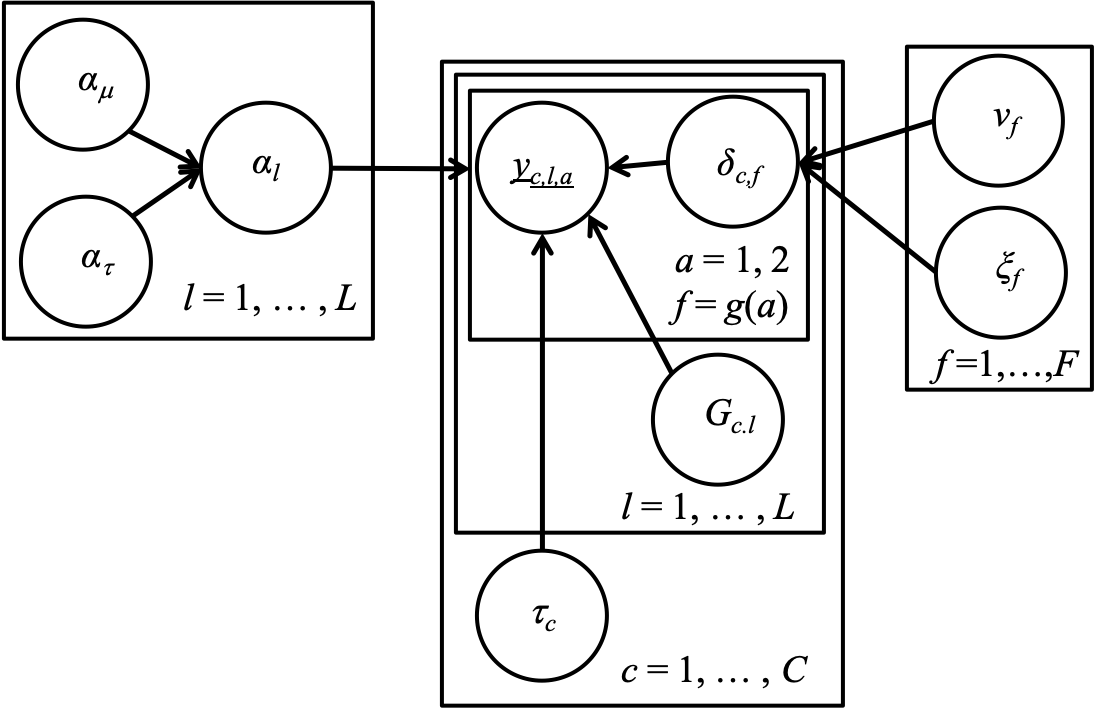
\includegraphics[width=0.25\linewidth]{g3} \caption{Model $g_2$}\label{fig:g3}
\end{figure}

Dye effects

\begin{Shaded}
\begin{Highlighting}[]
\KeywordTok{load}\NormalTok{(}\StringTok{"../systematic/g-3.Rda"}\NormalTok{)}
\NormalTok{g3.df =}\StringTok{ }\KeywordTok{data.frame}\NormalTok{(}\KeywordTok{as.matrix}\NormalTok{(sim.sample[[}\DecValTok{1}\NormalTok{]]))}

\NormalTok{lb =}\StringTok{ }\NormalTok{g3.df }\OperatorTok\StringTok{ }
\StringTok{    }\KeywordTok{select}\NormalTok{(}\KeywordTok{starts_with}\NormalTok{(}\StringTok{"gamma.dye"}\NormalTok{)) }\OperatorTok\StringTok{ }
\StringTok{    }\KeywordTok{summarise_all}\NormalTok{(quantile, }\DataTypeTok{prob =} \KeywordTok{c}\NormalTok{(}\FloatTok{0.025}\NormalTok{)) }\OperatorTok\StringTok{ }
\StringTok{  }\KeywordTok{unlist}\NormalTok{()}

\NormalTok{med =}\StringTok{ }\NormalTok{g3.df }\OperatorTok\StringTok{ }
\StringTok{  }\KeywordTok{select}\NormalTok{(}\KeywordTok{starts_with}\NormalTok{(}\StringTok{"gamma.dye"}\NormalTok{)) }\OperatorTok\StringTok{ }
\StringTok{  }\KeywordTok{summarise_all}\NormalTok{(quantile, }\DataTypeTok{prob =} \KeywordTok{c}\NormalTok{(}\FloatTok{0.5}\NormalTok{)) }\OperatorTok\StringTok{ }
\StringTok{  }\KeywordTok{unlist}\NormalTok{()}

\NormalTok{ub =}\StringTok{ }\NormalTok{g3.df }\OperatorTok\StringTok{ }
\StringTok{  }\KeywordTok{select}\NormalTok{(}\KeywordTok{starts_with}\NormalTok{(}\StringTok{"gamma.dye"}\NormalTok{)) }\OperatorTok\StringTok{ }
\StringTok{  }\KeywordTok{summarise_all}\NormalTok{(quantile, }\DataTypeTok{prob =} \KeywordTok{c}\NormalTok{(}\FloatTok{0.975}\NormalTok{)) }\OperatorTok\StringTok{ }
\StringTok{  }\KeywordTok{unlist}\NormalTok{()}

\NormalTok{quantiles.df =}\StringTok{ }\KeywordTok{data.frame}\NormalTok{(}\DataTypeTok{lb =}\NormalTok{ lb, }\DataTypeTok{med =}\NormalTok{ med, }\DataTypeTok{ub =}\NormalTok{ ub) }\OperatorTok\StringTok{ }
\StringTok{  }\KeywordTok{mutate}\NormalTok{(}\DataTypeTok{dye =} \DecValTok{1}\OperatorTok{:}\DecValTok{4}\NormalTok{)}

\NormalTok{p =}\StringTok{ }\KeywordTok{ggplot}\NormalTok{(}\DataTypeTok{data =}\NormalTok{ quantiles.df, }\KeywordTok{aes}\NormalTok{(}\DataTypeTok{x =}\NormalTok{ dye, }\DataTypeTok{y =}\NormalTok{ quantiles.df}\OperatorTok{$}\NormalTok{med)) }\OperatorTok{+}
\StringTok{  }\KeywordTok{geom_point}\NormalTok{(}\KeywordTok{aes}\NormalTok{(}\DataTypeTok{col =} \StringTok{"red"}\NormalTok{), }\DataTypeTok{show.legend =} \OtherTok{FALSE}\NormalTok{) }\OperatorTok{+}\StringTok{ }
\StringTok{  }\KeywordTok{geom_errorbar}\NormalTok{(}\KeywordTok{aes}\NormalTok{(}\DataTypeTok{ymin =}\NormalTok{ lb, }\DataTypeTok{ymax =}\NormalTok{ ub)) }\OperatorTok{+}
\StringTok{  }\KeywordTok{geom_hline}\NormalTok{(}\KeywordTok{aes}\NormalTok{(}\DataTypeTok{yintercept=}\DecValTok{0}\NormalTok{)) }\OperatorTok{+}
\StringTok{  }\KeywordTok{ylab}\NormalTok{(}\KeywordTok{bquote}\NormalTok{(gamma[dye])) }\OperatorTok{+}\StringTok{ }
\StringTok{  }\KeywordTok{xlab}\NormalTok{(}\StringTok{"Dye"}\NormalTok{)}
  
\NormalTok{p}
\end{Highlighting}
\end{Shaded}

\includegraphics{results_files/figure-latex/unnamed-chunk-16-1.pdf}

Plot the dye effects by Average Peak Height - no fitted line here
because with four points who cares:

\begin{Shaded}
\begin{Highlighting}[]
\NormalTok{aph =}\StringTok{ }\NormalTok{gNano.df }\OperatorTok\StringTok{ }
\StringTok{  }\KeywordTok{group_by}\NormalTok{(dye) }\OperatorTok\StringTok{ }
\StringTok{  }\KeywordTok{summarise}\NormalTok{(}\DataTypeTok{aph =} \KeywordTok{mean}\NormalTok{(}\KeywordTok{log}\NormalTok{(obs), }\DataTypeTok{na.rm =} \OtherTok{TRUE}\NormalTok{)) }\OperatorTok\StringTok{ }
\StringTok{  }\KeywordTok{pull}\NormalTok{(aph)}


\NormalTok{meanEffect =}\StringTok{ }\NormalTok{g3.df }\OperatorTok\StringTok{ }
\StringTok{  }\KeywordTok{select}\NormalTok{(}\KeywordTok{starts_with}\NormalTok{(}\StringTok{"gamma.dye"}\NormalTok{)) }\OperatorTok\StringTok{ }
\StringTok{  }\KeywordTok{summarise_all}\NormalTok{(mean, }\DataTypeTok{na.rm =} \OtherTok{TRUE}\NormalTok{) }\OperatorTok\StringTok{ }
\StringTok{  }\KeywordTok{unlist}\NormalTok{()}
  
\NormalTok{plot.df =}\StringTok{ }\KeywordTok{data.frame}\NormalTok{(}\DataTypeTok{aph =}\NormalTok{ aph, }\DataTypeTok{meanEffect =}\NormalTok{ meanEffect)}
\NormalTok{p =}\StringTok{ }\NormalTok{plot.df }\OperatorTok\StringTok{ }
\StringTok{  }\KeywordTok{ggplot}\NormalTok{(}\KeywordTok{aes}\NormalTok{(}\DataTypeTok{x =}\NormalTok{ aph, }\DataTypeTok{y =}\NormalTok{ meanEffect)) }\OperatorTok{+}\StringTok{ }
\StringTok{  }\KeywordTok{geom_point}\NormalTok{(}\DataTypeTok{show.legend =} \OtherTok{FALSE}\NormalTok{) }
\NormalTok{p}
\end{Highlighting}
\end{Shaded}

\includegraphics{results_files/figure-latex/unnamed-chunk-17-1.pdf}

Plot the observed vs the expected peak heights

\begin{Shaded}
\begin{Highlighting}[]
\NormalTok{expected =}\StringTok{ }\NormalTok{g3.df }\OperatorTok\StringTok{ }
\StringTok{  }\KeywordTok{select}\NormalTok{(}\KeywordTok{starts_with}\NormalTok{(}\StringTok{"pred"}\NormalTok{)) }\OperatorTok\StringTok{ }
\StringTok{  }\KeywordTok{summarise_all}\NormalTok{(mean) }\OperatorTok\StringTok{ }
\StringTok{  }\KeywordTok{unlist}\NormalTok{()}
  
\NormalTok{plot.df =}\StringTok{ }\KeywordTok{data.frame}\NormalTok{(}\DataTypeTok{observed =}\NormalTok{ gNano.df}\OperatorTok{$}\NormalTok{obs, }\DataTypeTok{expected =}\NormalTok{ expected)}
\NormalTok{p =}\StringTok{ }\NormalTok{plot.df }\OperatorTok\StringTok{ }
\StringTok{  }\KeywordTok{ggplot}\NormalTok{(}\KeywordTok{aes}\NormalTok{(}\DataTypeTok{x =} \KeywordTok{log10}\NormalTok{(observed), }\DataTypeTok{y =} \KeywordTok{log10}\NormalTok{(expected))) }\OperatorTok{+}
\StringTok{           }\KeywordTok{geom_point}\NormalTok{() }\OperatorTok{+}
\StringTok{           }\KeywordTok{geom_abline}\NormalTok{(}\KeywordTok{aes}\NormalTok{(}\DataTypeTok{intercept =} \DecValTok{0}\NormalTok{, }\DataTypeTok{slope =} \DecValTok{1}\NormalTok{)) }\OperatorTok{+}\StringTok{ }
\StringTok{          }\KeywordTok{xlim}\NormalTok{(}\DecValTok{2}\NormalTok{, }\DecValTok{5}\NormalTok{) }\OperatorTok{+}
\StringTok{          }\KeywordTok{ylim}\NormalTok{(}\DecValTok{2}\NormalTok{, }\DecValTok{5}\NormalTok{)}
\NormalTok{p}
\end{Highlighting}
\end{Shaded}

\begin{verbatim}
## Warning: Removed 8 rows containing missing values (geom_point).
\end{verbatim}

\includegraphics{results_files/figure-latex/unnamed-chunk-18-1.pdf}

\hypertarget{model-g_4---extra-variance}{%
\subsection{\texorpdfstring{Model \(g_4\) - extra
variance}{Model g\_4 - extra variance}}\label{model-g_4---extra-variance}}

Is the added variance being used?

\begin{Shaded}
\begin{Highlighting}[]
\KeywordTok{load}\NormalTok{(}\StringTok{"../systematic/g-4.Rda"}\NormalTok{)}
\NormalTok{g4.df =}\StringTok{ }\KeywordTok{data.frame}\NormalTok{(}\KeywordTok{as.matrix}\NormalTok{(sim.sample[[}\DecValTok{1}\NormalTok{]]))}

\NormalTok{g4.df =}\StringTok{ }\NormalTok{g4.df }\OperatorTok\StringTok{ }
\StringTok{  }\KeywordTok{mutate}\NormalTok{(}\DataTypeTok{sigma.sq0 =} \DecValTok{1} \OperatorTok{/}\StringTok{ }\NormalTok{tau0)}

\NormalTok{p =}\StringTok{ }\NormalTok{g4.df }\OperatorTok\StringTok{ }
\StringTok{  }\KeywordTok{ggplot}\NormalTok{(}\KeywordTok{aes}\NormalTok{(}\DataTypeTok{x =}\NormalTok{ sigma.sq0)) }\OperatorTok{+}
\StringTok{  }\KeywordTok{geom_density}\NormalTok{() }\OperatorTok{+}\StringTok{ }
\StringTok{  }\KeywordTok{xlab}\NormalTok{(}\KeywordTok{bquote}\NormalTok{(sigma[}\DecValTok{0}\NormalTok{]}\OperatorTok{^}\DecValTok{2}\NormalTok{))}

\NormalTok{p}
\end{Highlighting}
\end{Shaded}

\includegraphics{results_files/figure-latex/unnamed-chunk-19-1.pdf}

Plot the observed vs the expected peak heights

\begin{Shaded}
\begin{Highlighting}[]
\NormalTok{expected.g4 =}\StringTok{ }\NormalTok{g4.df }\OperatorTok\StringTok{ }
\StringTok{  }\KeywordTok{select}\NormalTok{(}\KeywordTok{starts_with}\NormalTok{(}\StringTok{"pred"}\NormalTok{)) }\OperatorTok\StringTok{ }
\StringTok{  }\KeywordTok{summarise_all}\NormalTok{(mean) }\OperatorTok\StringTok{ }
\StringTok{  }\KeywordTok{unlist}\NormalTok{()}
  
\NormalTok{plot.df =}\StringTok{ }\KeywordTok{data.frame}\NormalTok{(}\DataTypeTok{observed =}\NormalTok{ gNano.df}\OperatorTok{$}\NormalTok{obs, }\DataTypeTok{expected.g4 =}\NormalTok{ expected.g4, }\DataTypeTok{expected.g3 =}\NormalTok{ expected)}
\NormalTok{p =}\StringTok{ }\NormalTok{plot.df }\OperatorTok\StringTok{ }
\StringTok{  }\KeywordTok{ggplot}\NormalTok{(}\KeywordTok{aes}\NormalTok{(}\DataTypeTok{x =} \KeywordTok{log10}\NormalTok{(observed), }\DataTypeTok{y =} \KeywordTok{log10}\NormalTok{(expected.g4))) }\OperatorTok{+}
\StringTok{           }\KeywordTok{geom_point}\NormalTok{() }\OperatorTok{+}
\StringTok{           }\KeywordTok{geom_abline}\NormalTok{(}\KeywordTok{aes}\NormalTok{(}\DataTypeTok{intercept =} \DecValTok{0}\NormalTok{, }\DataTypeTok{slope =} \DecValTok{1}\NormalTok{)) }\OperatorTok{+}\StringTok{ }
\StringTok{          }\KeywordTok{xlim}\NormalTok{(}\DecValTok{2}\NormalTok{, }\DecValTok{5}\NormalTok{) }\OperatorTok{+}
\StringTok{          }\KeywordTok{ylim}\NormalTok{(}\DecValTok{2}\NormalTok{, }\DecValTok{5}\NormalTok{)}
\NormalTok{p}
\end{Highlighting}
\end{Shaded}

\begin{verbatim}
## Warning: Removed 8 rows containing missing values (geom_point).
\end{verbatim}

\includegraphics{results_files/figure-latex/unnamed-chunk-20-1.pdf}

Is it doing anything?

\begin{Shaded}
\begin{Highlighting}[]
\NormalTok{p =}\StringTok{ }\NormalTok{plot.df }\OperatorTok\StringTok{ }
\StringTok{  }\KeywordTok{ggplot}\NormalTok{(}\KeywordTok{aes}\NormalTok{(}\DataTypeTok{x =} \KeywordTok{log10}\NormalTok{(expected.g3), }\DataTypeTok{y =} \KeywordTok{log10}\NormalTok{(expected.g4))) }\OperatorTok{+}
\StringTok{           }\KeywordTok{geom_point}\NormalTok{() }\OperatorTok{+}
\StringTok{           }\KeywordTok{geom_abline}\NormalTok{(}\KeywordTok{aes}\NormalTok{(}\DataTypeTok{intercept =} \DecValTok{0}\NormalTok{, }\DataTypeTok{slope =} \DecValTok{1}\NormalTok{)) }\OperatorTok{+}\StringTok{ }
\StringTok{          }\KeywordTok{xlim}\NormalTok{(}\DecValTok{2}\NormalTok{, }\DecValTok{5}\NormalTok{) }\OperatorTok{+}
\StringTok{          }\KeywordTok{ylim}\NormalTok{(}\DecValTok{2}\NormalTok{, }\DecValTok{5}\NormalTok{)}
\NormalTok{p}
\end{Highlighting}
\end{Shaded}

\includegraphics{results_files/figure-latex/unnamed-chunk-21-1.pdf}

I think it's doing what it is supposed to.

Let's try and look at the expected values slightly differently. I will
work with the summary stats rather than the raw data

\begin{Shaded}
\begin{Highlighting}[]
\KeywordTok{load}\NormalTok{(}\StringTok{"../systematic/g-3.Rda"}\NormalTok{)}

\NormalTok{g3.quantiles =}\StringTok{ }\KeywordTok{as.data.frame}\NormalTok{(}\KeywordTok{t}\NormalTok{(simSummary}\OperatorTok{$}\NormalTok{quantiles)) }\OperatorTok\StringTok{ }
\StringTok{  }\KeywordTok{select}\NormalTok{(}\KeywordTok{starts_with}\NormalTok{(}\StringTok{"pred"}\NormalTok{))  }\OperatorTok
\StringTok{   }\NormalTok{rownames_to_column }\OperatorTok\StringTok{ }
\StringTok{   }\KeywordTok{gather}\NormalTok{(var, value, }\OperatorTok{-}\NormalTok{rowname) }\OperatorTok\StringTok{ }
\StringTok{   }\KeywordTok{spread}\NormalTok{(rowname, value) }\OperatorTok\StringTok{ }
\StringTok{  }\KeywordTok{mutate}\NormalTok{(}\DataTypeTok{var =} \KeywordTok{as.numeric}\NormalTok{(}\KeywordTok{gsub}\NormalTok{(}\StringTok{"^pred}\CharTok{\textbackslash{}\textbackslash{}}\StringTok{[([0-9]+)}\CharTok{\textbackslash{}\textbackslash{}}\StringTok{]$"}\NormalTok{, }\StringTok{"}\CharTok{\textbackslash{}\textbackslash{}}\StringTok{1"}\NormalTok{, var))) }\OperatorTok\StringTok{ }
\StringTok{  }\KeywordTok{arrange}\NormalTok{(var)}

\NormalTok{g3.stats =}\StringTok{ }\KeywordTok{as.data.frame}\NormalTok{(}\KeywordTok{t}\NormalTok{(simSummary}\OperatorTok{$}\NormalTok{statistics)) }\OperatorTok\StringTok{ }
\StringTok{  }\KeywordTok{select}\NormalTok{(}\KeywordTok{starts_with}\NormalTok{(}\StringTok{"pred"}\NormalTok{))  }\OperatorTok
\StringTok{   }\NormalTok{rownames_to_column }\OperatorTok\StringTok{ }
\StringTok{   }\KeywordTok{gather}\NormalTok{(var, value, }\OperatorTok{-}\NormalTok{rowname) }\OperatorTok\StringTok{ }
\StringTok{   }\KeywordTok{spread}\NormalTok{(rowname, value) }\OperatorTok\StringTok{ }
\StringTok{  }\KeywordTok{mutate}\NormalTok{(}\DataTypeTok{var =} \KeywordTok{as.numeric}\NormalTok{(}\KeywordTok{gsub}\NormalTok{(}\StringTok{"^pred}\CharTok{\textbackslash{}\textbackslash{}}\StringTok{[([0-9]+)}\CharTok{\textbackslash{}\textbackslash{}}\StringTok{]$"}\NormalTok{, }\StringTok{"}\CharTok{\textbackslash{}\textbackslash{}}\StringTok{1"}\NormalTok{, var))) }\OperatorTok\StringTok{ }
\StringTok{  }\KeywordTok{arrange}\NormalTok{(var)}



\KeywordTok{load}\NormalTok{(}\StringTok{"../systematic/g-4.Rda"}\NormalTok{)}

\NormalTok{g4.quantiles =}\StringTok{ }\KeywordTok{as.data.frame}\NormalTok{(}\KeywordTok{t}\NormalTok{(simSummary}\OperatorTok{$}\NormalTok{quantiles)) }\OperatorTok\StringTok{ }
\StringTok{    }\KeywordTok{select}\NormalTok{(}\KeywordTok{starts_with}\NormalTok{(}\StringTok{"pred"}\NormalTok{))  }\OperatorTok
\StringTok{   }\NormalTok{rownames_to_column }\OperatorTok\StringTok{ }
\StringTok{   }\KeywordTok{gather}\NormalTok{(var, value, }\OperatorTok{-}\NormalTok{rowname) }\OperatorTok\StringTok{ }
\StringTok{   }\KeywordTok{spread}\NormalTok{(rowname, value)  }\OperatorTok\StringTok{ }
\StringTok{  }\KeywordTok{mutate}\NormalTok{(}\DataTypeTok{var =} \KeywordTok{as.numeric}\NormalTok{(}\KeywordTok{gsub}\NormalTok{(}\StringTok{"^pred}\CharTok{\textbackslash{}\textbackslash{}}\StringTok{[([0-9]+)}\CharTok{\textbackslash{}\textbackslash{}}\StringTok{]$"}\NormalTok{, }\StringTok{"}\CharTok{\textbackslash{}\textbackslash{}}\StringTok{1"}\NormalTok{, var))) }\OperatorTok\StringTok{ }
\StringTok{  }\KeywordTok{arrange}\NormalTok{(var)}

\NormalTok{plot.df =}\StringTok{ }\KeywordTok{bind_rows}\NormalTok{(g3.quantiles, g4.quantiles) }\OperatorTok\StringTok{ }
\StringTok{  }\KeywordTok{mutate}\NormalTok{(}\DataTypeTok{model =} \KeywordTok{rep}\NormalTok{(}\KeywordTok{c}\NormalTok{(}\StringTok{"g3"}\NormalTok{, }\StringTok{"g4"}\NormalTok{), }\KeywordTok{rep}\NormalTok{(}\KeywordTok{nrow}\NormalTok{(g3.quantiles), }\DecValTok{2}\NormalTok{))) }\OperatorTok\StringTok{ }
\StringTok{  }\KeywordTok{mutate}\NormalTok{(}\DataTypeTok{obs =} \KeywordTok{rep}\NormalTok{(gNano.df}\OperatorTok{$}\NormalTok{obs, }\DecValTok{2}\NormalTok{)) }\OperatorTok\StringTok{ }
\StringTok{  }\KeywordTok{rename}\NormalTok{(}\DataTypeTok{med =} \StringTok{`}\DataTypeTok{50%}\StringTok{`}\NormalTok{, }\DataTypeTok{lb =} \StringTok{`}\DataTypeTok{2.5%}\StringTok{`}\NormalTok{, }\DataTypeTok{ub =} \StringTok{`}\DataTypeTok{97.5%}\StringTok{`}\NormalTok{) }\OperatorTok\StringTok{ }
\StringTok{  }\KeywordTok{select}\NormalTok{(obs, model, lb, med, ub) }\OperatorTok\StringTok{ }
\StringTok{  }\KeywordTok{arrange}\NormalTok{(obs)}


\NormalTok{p =}\StringTok{ }\NormalTok{plot.df }\OperatorTok\StringTok{ }
\StringTok{  }\KeywordTok{ggplot}\NormalTok{(}\KeywordTok{aes}\NormalTok{(}\DataTypeTok{x =} \KeywordTok{log10}\NormalTok{(obs), }\DataTypeTok{y =} \KeywordTok{log10}\NormalTok{(med))) }\OperatorTok{+}
\StringTok{  }\KeywordTok{facet_grid}\NormalTok{(}\KeywordTok{vars}\NormalTok{(model)) }\OperatorTok{+}
\StringTok{    }\KeywordTok{geom_abline}\NormalTok{(}\KeywordTok{aes}\NormalTok{(}\DataTypeTok{intercept =} \DecValTok{0}\NormalTok{, }\DataTypeTok{slope =} \DecValTok{1}\NormalTok{)) }\OperatorTok{+}
\StringTok{    }\KeywordTok{xlim}\NormalTok{(}\DecValTok{2}\NormalTok{, }\DecValTok{5}\NormalTok{) }\OperatorTok{+}
\StringTok{    }\KeywordTok{ylim}\NormalTok{(}\DecValTok{2}\NormalTok{, }\DecValTok{5}\NormalTok{) }\OperatorTok{+}
\StringTok{  }\KeywordTok{geom_point}\NormalTok{(}\DataTypeTok{show.legend =} \OtherTok{FALSE}\NormalTok{) }\OperatorTok{+}\StringTok{ }
\StringTok{  }\KeywordTok{geom_smooth}\NormalTok{() }\OperatorTok{+}
\StringTok{  }\KeywordTok{geom_line}\NormalTok{(}\KeywordTok{aes}\NormalTok{(}\DataTypeTok{y =} \KeywordTok{log10}\NormalTok{(lb)), }\DataTypeTok{col =} \StringTok{"green"}\NormalTok{) }\OperatorTok{+}\StringTok{ }\KeywordTok{geom_line}\NormalTok{(}\KeywordTok{aes}\NormalTok{(}\DataTypeTok{y =} \KeywordTok{log10}\NormalTok{(ub)), }\DataTypeTok{col =} \StringTok{"red"}\NormalTok{)}
\NormalTok{p}
\end{Highlighting}
\end{Shaded}

\begin{verbatim}
## Warning: Removed 128 rows containing non-finite values (stat_smooth).
\end{verbatim}

\begin{verbatim}
## Warning: Removed 128 rows containing missing values (geom_point).
\end{verbatim}

\begin{verbatim}
## Warning: Removed 39 rows containing missing values (geom_path).
\end{verbatim}

\begin{verbatim}
## Warning: Removed 8 rows containing missing values (geom_path).
\end{verbatim}

\includegraphics{results_files/figure-latex/unnamed-chunk-22-1.pdf}

Now we move on the the log normal models

\hypertarget{model-ln_0---no-effects}{%
\subsection{\texorpdfstring{Model \(ln_0\) - no
effects}{Model ln\_0 - no effects}}\label{model-ln_0---no-effects}}

Tau

\begin{Shaded}
\begin{Highlighting}[]
\KeywordTok{load}\NormalTok{(}\StringTok{"../systematic/ln-0.Rda"}\NormalTok{)}
\NormalTok{ln0.df =}\StringTok{ }\KeywordTok{data.frame}\NormalTok{(}\KeywordTok{as.matrix}\NormalTok{(sim.sample[[}\DecValTok{1}\NormalTok{]]))}

\NormalTok{p =}\StringTok{ }\NormalTok{ln0.df }\OperatorTok\StringTok{ }
\StringTok{  }\KeywordTok{ggplot}\NormalTok{(}\KeywordTok{aes}\NormalTok{(}\DataTypeTok{x =}\NormalTok{ tau)) }\OperatorTok{+}
\StringTok{  }\KeywordTok{geom_density}\NormalTok{()}
\NormalTok{p}
\end{Highlighting}
\end{Shaded}

\includegraphics{results_files/figure-latex/unnamed-chunk-23-1.pdf}

Mu

\begin{Shaded}
\begin{Highlighting}[]
\NormalTok{p =}\StringTok{ }\NormalTok{ln0.df }\OperatorTok\StringTok{ }
\StringTok{  }\KeywordTok{ggplot}\NormalTok{(}\KeywordTok{aes}\NormalTok{(}\DataTypeTok{x =}\NormalTok{ Mu)) }\OperatorTok{+}
\StringTok{  }\KeywordTok{geom_density}\NormalTok{()}
\NormalTok{p}
\end{Highlighting}
\end{Shaded}

\includegraphics{results_files/figure-latex/unnamed-chunk-24-1.pdf}

Comparing expected and observed peak heights

\begin{Shaded}
\begin{Highlighting}[]
\KeywordTok{library}\NormalTok{(gNanoPkg)}
\NormalTok{gNano.df =}\StringTok{ }\KeywordTok{readData}\NormalTok{()}
\NormalTok{expected =}\StringTok{ }\NormalTok{ln0.df }\OperatorTok\StringTok{ }
\StringTok{  }\KeywordTok{select}\NormalTok{(}\KeywordTok{starts_with}\NormalTok{(}\StringTok{"pred"}\NormalTok{)) }\OperatorTok\StringTok{ }
\StringTok{  }\KeywordTok{summarise_all}\NormalTok{(mean) }\OperatorTok\StringTok{ }
\StringTok{  }\KeywordTok{unlist}\NormalTok{()}
  
\NormalTok{plot.df =}\StringTok{ }\KeywordTok{data.frame}\NormalTok{(}\DataTypeTok{observed =}\NormalTok{ gNano.df}\OperatorTok{$}\NormalTok{obs, }\DataTypeTok{expected =}\NormalTok{ expected)}
\NormalTok{p =}\StringTok{ }\NormalTok{plot.df }\OperatorTok\StringTok{ }
\StringTok{  }\KeywordTok{ggplot}\NormalTok{(}\KeywordTok{aes}\NormalTok{(}\DataTypeTok{x =} \KeywordTok{log10}\NormalTok{(observed), }\DataTypeTok{y =} \KeywordTok{log10}\NormalTok{(expected))) }\OperatorTok{+}
\StringTok{           }\KeywordTok{geom_point}\NormalTok{() }\OperatorTok{+}
\StringTok{           }\KeywordTok{geom_abline}\NormalTok{(}\KeywordTok{aes}\NormalTok{(}\DataTypeTok{intercept =} \DecValTok{0}\NormalTok{, }\DataTypeTok{slope =} \DecValTok{1}\NormalTok{)) }\OperatorTok{+}\StringTok{ }
\StringTok{          }\KeywordTok{xlim}\NormalTok{(}\DecValTok{0}\NormalTok{, }\DecValTok{5}\NormalTok{) }\OperatorTok{+}
\StringTok{          }\KeywordTok{ylim}\NormalTok{(}\DecValTok{0}\NormalTok{, }\DecValTok{5}\NormalTok{)}
\NormalTok{p}
\end{Highlighting}
\end{Shaded}

\includegraphics{results_files/figure-latex/unnamed-chunk-25-1.pdf}

\hypertarget{model-ln_1---profile-effects}{%
\subsection{\texorpdfstring{Model \(ln_1\) - profile
effects}{Model ln\_1 - profile effects}}\label{model-ln_1---profile-effects}}

Load the data

\begin{Shaded}
\begin{Highlighting}[]
\KeywordTok{load}\NormalTok{(}\StringTok{"../systematic/ln-1.Rda"}\NormalTok{)}
\NormalTok{ln1.df =}\StringTok{ }\KeywordTok{as.data.frame}\NormalTok{(}\KeywordTok{as.matrix}\NormalTok{(sim.sample))}
\end{Highlighting}
\end{Shaded}

Showing the per profile effects

\begin{Shaded}
\begin{Highlighting}[]
\NormalTok{lb =}\StringTok{ }\NormalTok{ln1.df }\OperatorTok\StringTok{ }
\StringTok{    }\KeywordTok{select}\NormalTok{(}\KeywordTok{starts_with}\NormalTok{(}\StringTok{"beta.profile"}\NormalTok{)) }\OperatorTok\StringTok{ }
\StringTok{    }\KeywordTok{summarise_all}\NormalTok{(quantile, }\DataTypeTok{prob =} \KeywordTok{c}\NormalTok{(}\FloatTok{0.025}\NormalTok{)) }\OperatorTok\StringTok{ }
\StringTok{  }\KeywordTok{unlist}\NormalTok{()}

\NormalTok{med =}\StringTok{ }\NormalTok{ln1.df }\OperatorTok\StringTok{ }
\StringTok{  }\KeywordTok{select}\NormalTok{(}\KeywordTok{starts_with}\NormalTok{(}\StringTok{"beta.profile"}\NormalTok{)) }\OperatorTok\StringTok{ }
\StringTok{  }\KeywordTok{summarise_all}\NormalTok{(quantile, }\DataTypeTok{prob =} \KeywordTok{c}\NormalTok{(}\FloatTok{0.5}\NormalTok{)) }\OperatorTok\StringTok{ }
\StringTok{  }\KeywordTok{unlist}\NormalTok{()}

\NormalTok{ub =}\StringTok{ }\NormalTok{ln1.df }\OperatorTok\StringTok{ }
\StringTok{  }\KeywordTok{select}\NormalTok{(}\KeywordTok{starts_with}\NormalTok{(}\StringTok{"beta.profile"}\NormalTok{)) }\OperatorTok\StringTok{ }
\StringTok{  }\KeywordTok{summarise_all}\NormalTok{(quantile, }\DataTypeTok{prob =} \KeywordTok{c}\NormalTok{(}\FloatTok{0.975}\NormalTok{)) }\OperatorTok\StringTok{ }
\StringTok{  }\KeywordTok{unlist}\NormalTok{()}

\NormalTok{quantiles.df =}\StringTok{ }\KeywordTok{data.frame}\NormalTok{(}\DataTypeTok{lb =}\NormalTok{ lb, }\DataTypeTok{med =}\NormalTok{ med, }\DataTypeTok{ub =}\NormalTok{ ub) }\OperatorTok\StringTok{ }
\StringTok{  }\KeywordTok{mutate}\NormalTok{(}\DataTypeTok{profile =} \DecValTok{1}\OperatorTok{:}\DecValTok{102}\NormalTok{)}

\NormalTok{p =}\StringTok{ }\KeywordTok{ggplot}\NormalTok{(}\DataTypeTok{data =}\NormalTok{ quantiles.df, }\KeywordTok{aes}\NormalTok{(}\DataTypeTok{x =}\NormalTok{ profile, }\DataTypeTok{y =}\NormalTok{ quantiles.df}\OperatorTok{$}\NormalTok{med)) }\OperatorTok{+}
\StringTok{  }\KeywordTok{geom_point}\NormalTok{(}\KeywordTok{aes}\NormalTok{(}\DataTypeTok{col =} \StringTok{"red"}\NormalTok{), }\DataTypeTok{show.legend =} \OtherTok{FALSE}\NormalTok{) }\OperatorTok{+}\StringTok{ }
\StringTok{  }\KeywordTok{geom_errorbar}\NormalTok{(}\KeywordTok{aes}\NormalTok{(}\DataTypeTok{ymin =}\NormalTok{ lb, }\DataTypeTok{ymax =}\NormalTok{ ub)) }\OperatorTok{+}
\StringTok{  }\KeywordTok{geom_hline}\NormalTok{(}\KeywordTok{aes}\NormalTok{(}\DataTypeTok{yintercept=}\DecValTok{0}\NormalTok{)) }\OperatorTok{+}
\StringTok{  }\KeywordTok{ylab}\NormalTok{(}\KeywordTok{bquote}\NormalTok{(beta[Profile])) }\OperatorTok{+}\StringTok{ }
\StringTok{  }\KeywordTok{xlab}\NormalTok{(}\StringTok{"Profile"}\NormalTok{)}
  
\NormalTok{p}
\end{Highlighting}
\end{Shaded}

\includegraphics{results_files/figure-latex/unnamed-chunk-27-1.pdf}

Now showing the relationship between profile aph and profile effects
from model

\begin{Shaded}
\begin{Highlighting}[]
\NormalTok{aph =}\StringTok{ }\NormalTok{gNano.df }\OperatorTok\StringTok{ }
\StringTok{  }\KeywordTok{group_by}\NormalTok{(prof) }\OperatorTok\StringTok{ }
\StringTok{  }\KeywordTok{summarise}\NormalTok{(}\DataTypeTok{aph =} \KeywordTok{mean}\NormalTok{(}\KeywordTok{log}\NormalTok{(obs), }\DataTypeTok{na.rm =} \OtherTok{TRUE}\NormalTok{)) }\OperatorTok\StringTok{ }
\StringTok{  }\KeywordTok{pull}\NormalTok{(aph)}


\NormalTok{meanEffect =}\StringTok{ }\NormalTok{ln1.df }\OperatorTok\StringTok{ }
\StringTok{  }\KeywordTok{select}\NormalTok{(}\KeywordTok{starts_with}\NormalTok{(}\StringTok{"beta.profile"}\NormalTok{)) }\OperatorTok\StringTok{ }
\StringTok{  }\KeywordTok{summarise_all}\NormalTok{(mean, }\DataTypeTok{na.rm =} \OtherTok{TRUE}\NormalTok{) }\OperatorTok\StringTok{ }
\StringTok{  }\KeywordTok{unlist}\NormalTok{()}
  
\NormalTok{plot.df =}\StringTok{ }\KeywordTok{data.frame}\NormalTok{(}\DataTypeTok{aph =}\NormalTok{ aph, }\DataTypeTok{meanEffect =}\NormalTok{ meanEffect)}
\NormalTok{p =}\StringTok{ }\NormalTok{plot.df }\OperatorTok\StringTok{ }
\StringTok{  }\KeywordTok{ggplot}\NormalTok{(}\KeywordTok{aes}\NormalTok{(}\DataTypeTok{x =}\NormalTok{ aph, }\DataTypeTok{y =}\NormalTok{ meanEffect)) }\OperatorTok{+}\StringTok{ }
\StringTok{  }\KeywordTok{geom_point}\NormalTok{(}\DataTypeTok{show.legend =} \OtherTok{FALSE}\NormalTok{) }\OperatorTok{+}
\StringTok{  }\KeywordTok{geom_smooth}\NormalTok{()}

\NormalTok{p}
\end{Highlighting}
\end{Shaded}

\includegraphics{results_files/figure-latex/unnamed-chunk-28-1.pdf}

Plotting observed vs expected peak heights

\begin{Shaded}
\begin{Highlighting}[]
\NormalTok{expected =}\StringTok{ }\NormalTok{ln1.df }\OperatorTok\StringTok{ }
\StringTok{  }\KeywordTok{select}\NormalTok{(}\KeywordTok{starts_with}\NormalTok{(}\StringTok{"pred"}\NormalTok{)) }\OperatorTok\StringTok{ }
\StringTok{  }\KeywordTok{summarise_all}\NormalTok{(mean) }\OperatorTok\StringTok{ }
\StringTok{  }\KeywordTok{unlist}\NormalTok{()}
  
\NormalTok{plot.df =}\StringTok{ }\KeywordTok{data.frame}\NormalTok{(}\DataTypeTok{observed =}\NormalTok{ gNano.df}\OperatorTok{$}\NormalTok{obs, }\DataTypeTok{expected =}\NormalTok{ expected)}
\NormalTok{p =}\StringTok{ }\NormalTok{plot.df }\OperatorTok\StringTok{ }
\StringTok{  }\KeywordTok{ggplot}\NormalTok{(}\KeywordTok{aes}\NormalTok{(}\DataTypeTok{x =} \KeywordTok{log10}\NormalTok{(observed), }\DataTypeTok{y =} \KeywordTok{log10}\NormalTok{(expected))) }\OperatorTok{+}
\StringTok{           }\KeywordTok{geom_point}\NormalTok{() }\OperatorTok{+}
\StringTok{           }\KeywordTok{geom_abline}\NormalTok{(}\KeywordTok{aes}\NormalTok{(}\DataTypeTok{intercept =} \DecValTok{0}\NormalTok{, }\DataTypeTok{slope =} \DecValTok{1}\NormalTok{)) }\OperatorTok{+}\StringTok{ }
\StringTok{          }\KeywordTok{xlim}\NormalTok{(}\DecValTok{0}\NormalTok{, }\DecValTok{5}\NormalTok{) }\OperatorTok{+}
\StringTok{          }\KeywordTok{ylim}\NormalTok{(}\DecValTok{0}\NormalTok{, }\DecValTok{5}\NormalTok{)}
\NormalTok{p}
\end{Highlighting}
\end{Shaded}

\includegraphics{results_files/figure-latex/unnamed-chunk-29-1.pdf}

\hypertarget{model-ln_2---locus-effects}{%
\subsection{\texorpdfstring{Model \(ln_2\) - locus
effects}{Model ln\_2 - locus effects}}\label{model-ln_2---locus-effects}}

\begin{Shaded}
\begin{Highlighting}[]
\KeywordTok{load}\NormalTok{(}\StringTok{"../systematic/ln-2.Rda"}\NormalTok{)}
\NormalTok{ln2.df =}\StringTok{ }\KeywordTok{data.frame}\NormalTok{(}\KeywordTok{as.matrix}\NormalTok{(sim.sample[[}\DecValTok{1}\NormalTok{]]))}

\NormalTok{lb =}\StringTok{ }\NormalTok{ln2.df }\OperatorTok\StringTok{ }
\StringTok{    }\KeywordTok{select}\NormalTok{(}\KeywordTok{starts_with}\NormalTok{(}\StringTok{"alpha.locus"}\NormalTok{)) }\OperatorTok\StringTok{ }
\StringTok{    }\KeywordTok{summarise_all}\NormalTok{(quantile, }\DataTypeTok{prob =} \KeywordTok{c}\NormalTok{(}\FloatTok{0.025}\NormalTok{)) }\OperatorTok\StringTok{ }
\StringTok{  }\KeywordTok{unlist}\NormalTok{()}

\NormalTok{med =}\StringTok{ }\NormalTok{ln2.df }\OperatorTok\StringTok{ }
\StringTok{  }\KeywordTok{select}\NormalTok{(}\KeywordTok{starts_with}\NormalTok{(}\StringTok{"alpha.locus"}\NormalTok{)) }\OperatorTok\StringTok{ }
\StringTok{  }\KeywordTok{summarise_all}\NormalTok{(quantile, }\DataTypeTok{prob =} \KeywordTok{c}\NormalTok{(}\FloatTok{0.5}\NormalTok{)) }\OperatorTok\StringTok{ }
\StringTok{  }\KeywordTok{unlist}\NormalTok{()}

\NormalTok{ub =}\StringTok{ }\NormalTok{ln2.df }\OperatorTok\StringTok{ }
\StringTok{  }\KeywordTok{select}\NormalTok{(}\KeywordTok{starts_with}\NormalTok{(}\StringTok{"alpha.locus"}\NormalTok{)) }\OperatorTok\StringTok{ }
\StringTok{  }\KeywordTok{summarise_all}\NormalTok{(quantile, }\DataTypeTok{prob =} \KeywordTok{c}\NormalTok{(}\FloatTok{0.975}\NormalTok{)) }\OperatorTok\StringTok{ }
\StringTok{  }\KeywordTok{unlist}\NormalTok{()}

\NormalTok{quantiles.df =}\StringTok{ }\KeywordTok{data.frame}\NormalTok{(}\DataTypeTok{lb =}\NormalTok{ lb, }\DataTypeTok{med =}\NormalTok{ med, }\DataTypeTok{ub =}\NormalTok{ ub) }\OperatorTok\StringTok{ }
\StringTok{  }\KeywordTok{mutate}\NormalTok{(}\DataTypeTok{locus =} \DecValTok{1}\OperatorTok{:}\DecValTok{31}\NormalTok{)}

\NormalTok{p =}\StringTok{ }\KeywordTok{ggplot}\NormalTok{(}\DataTypeTok{data =}\NormalTok{ quantiles.df, }\KeywordTok{aes}\NormalTok{(}\DataTypeTok{x =}\NormalTok{ locus, }\DataTypeTok{y =}\NormalTok{ quantiles.df}\OperatorTok{$}\NormalTok{med)) }\OperatorTok{+}
\StringTok{  }\KeywordTok{geom_point}\NormalTok{(}\KeywordTok{aes}\NormalTok{(}\DataTypeTok{col =} \StringTok{"red"}\NormalTok{), }\DataTypeTok{show.legend =} \OtherTok{FALSE}\NormalTok{) }\OperatorTok{+}\StringTok{ }
\StringTok{  }\KeywordTok{geom_errorbar}\NormalTok{(}\KeywordTok{aes}\NormalTok{(}\DataTypeTok{ymin =}\NormalTok{ lb, }\DataTypeTok{ymax =}\NormalTok{ ub)) }\OperatorTok{+}
\StringTok{  }\KeywordTok{geom_hline}\NormalTok{(}\KeywordTok{aes}\NormalTok{(}\DataTypeTok{yintercept=}\DecValTok{0}\NormalTok{)) }\OperatorTok{+}
\StringTok{  }\KeywordTok{ylab}\NormalTok{(}\KeywordTok{bquote}\NormalTok{(alpha[locus])) }\OperatorTok{+}\StringTok{ }
\StringTok{  }\KeywordTok{xlab}\NormalTok{(}\StringTok{"Locus"}\NormalTok{)}
  
\NormalTok{p}
\end{Highlighting}
\end{Shaded}

\includegraphics{results_files/figure-latex/unnamed-chunk-30-1.pdf}

Plot the observed vs the expected peak heights

\begin{Shaded}
\begin{Highlighting}[]
\NormalTok{expected =}\StringTok{ }\NormalTok{ln2.df }\OperatorTok\StringTok{ }
\StringTok{  }\KeywordTok{select}\NormalTok{(}\KeywordTok{starts_with}\NormalTok{(}\StringTok{"pred"}\NormalTok{)) }\OperatorTok\StringTok{ }
\StringTok{  }\KeywordTok{summarise_all}\NormalTok{(mean) }\OperatorTok\StringTok{ }
\StringTok{  }\KeywordTok{unlist}\NormalTok{()}
  
\NormalTok{plot.df =}\StringTok{ }\KeywordTok{data.frame}\NormalTok{(}\DataTypeTok{observed =}\NormalTok{ gNano.df}\OperatorTok{$}\NormalTok{obs, }\DataTypeTok{expected =}\NormalTok{ expected)}
\NormalTok{p =}\StringTok{ }\NormalTok{plot.df }\OperatorTok\StringTok{ }
\StringTok{  }\KeywordTok{ggplot}\NormalTok{(}\KeywordTok{aes}\NormalTok{(}\DataTypeTok{x =} \KeywordTok{log10}\NormalTok{(observed), }\DataTypeTok{y =} \KeywordTok{log10}\NormalTok{(expected))) }\OperatorTok{+}
\StringTok{           }\KeywordTok{geom_point}\NormalTok{() }\OperatorTok{+}
\StringTok{           }\KeywordTok{geom_abline}\NormalTok{(}\KeywordTok{aes}\NormalTok{(}\DataTypeTok{intercept =} \DecValTok{0}\NormalTok{, }\DataTypeTok{slope =} \DecValTok{1}\NormalTok{)) }\OperatorTok{+}\StringTok{ }
\StringTok{          }\KeywordTok{xlim}\NormalTok{(}\DecValTok{0}\NormalTok{, }\DecValTok{5}\NormalTok{) }\OperatorTok{+}
\StringTok{          }\KeywordTok{ylim}\NormalTok{(}\DecValTok{0}\NormalTok{, }\DecValTok{5}\NormalTok{)}
\NormalTok{p}
\end{Highlighting}
\end{Shaded}

\includegraphics{results_files/figure-latex/unnamed-chunk-31-1.pdf}

Plot the locus effects by Average Peak Height:

\begin{Shaded}
\begin{Highlighting}[]
\NormalTok{aph =}\StringTok{ }\NormalTok{gNano.df }\OperatorTok\StringTok{ }
\StringTok{  }\KeywordTok{group_by}\NormalTok{(loc) }\OperatorTok\StringTok{ }
\StringTok{  }\KeywordTok{summarise}\NormalTok{(}\DataTypeTok{aph =} \KeywordTok{mean}\NormalTok{(}\KeywordTok{log}\NormalTok{(obs), }\DataTypeTok{na.rm =} \OtherTok{TRUE}\NormalTok{)) }\OperatorTok\StringTok{ }
\StringTok{  }\KeywordTok{pull}\NormalTok{(aph)}


\NormalTok{meanEffect =}\StringTok{ }\NormalTok{ln2.df }\OperatorTok\StringTok{ }
\StringTok{  }\KeywordTok{select}\NormalTok{(}\KeywordTok{starts_with}\NormalTok{(}\StringTok{"alpha.locus"}\NormalTok{)) }\OperatorTok\StringTok{ }
\StringTok{  }\KeywordTok{summarise_all}\NormalTok{(mean, }\DataTypeTok{na.rm =} \OtherTok{TRUE}\NormalTok{) }\OperatorTok\StringTok{ }
\StringTok{  }\KeywordTok{unlist}\NormalTok{()}
  
\NormalTok{plot.df =}\StringTok{ }\KeywordTok{data.frame}\NormalTok{(}\DataTypeTok{aph =}\NormalTok{ aph, }\DataTypeTok{meanEffect =}\NormalTok{ meanEffect)}
\NormalTok{p =}\StringTok{ }\NormalTok{plot.df }\OperatorTok\StringTok{ }
\StringTok{  }\KeywordTok{ggplot}\NormalTok{(}\KeywordTok{aes}\NormalTok{(}\DataTypeTok{x =}\NormalTok{ aph, }\DataTypeTok{y =}\NormalTok{ meanEffect)) }\OperatorTok{+}\StringTok{ }
\StringTok{  }\KeywordTok{geom_point}\NormalTok{(}\DataTypeTok{show.legend =} \OtherTok{FALSE}\NormalTok{) }\OperatorTok{+}
\StringTok{  }\KeywordTok{geom_smooth}\NormalTok{()}

\NormalTok{p}
\end{Highlighting}
\end{Shaded}

\includegraphics{results_files/figure-latex/unnamed-chunk-32-1.pdf}

\hypertarget{model-ln_3---all-other-effects-except-extra-variance}{%
\subsection{\texorpdfstring{Model \(ln_3\) - all other effects except
extra
variance}{Model ln\_3 - all other effects except extra variance}}\label{model-ln_3---all-other-effects-except-extra-variance}}

Dye effects

\begin{Shaded}
\begin{Highlighting}[]
\KeywordTok{load}\NormalTok{(}\StringTok{"../systematic/g-3.Rda"}\NormalTok{)}
\NormalTok{ln3.df =}\StringTok{ }\KeywordTok{data.frame}\NormalTok{(}\KeywordTok{as.matrix}\NormalTok{(sim.sample[[}\DecValTok{1}\NormalTok{]]))}

\NormalTok{lb =}\StringTok{ }\NormalTok{ln3.df }\OperatorTok\StringTok{ }
\StringTok{    }\KeywordTok{select}\NormalTok{(}\KeywordTok{starts_with}\NormalTok{(}\StringTok{"gamma.dye"}\NormalTok{)) }\OperatorTok\StringTok{ }
\StringTok{    }\KeywordTok{summarise_all}\NormalTok{(quantile, }\DataTypeTok{prob =} \KeywordTok{c}\NormalTok{(}\FloatTok{0.025}\NormalTok{)) }\OperatorTok\StringTok{ }
\StringTok{  }\KeywordTok{unlist}\NormalTok{()}

\NormalTok{med =}\StringTok{ }\NormalTok{ln3.df }\OperatorTok\StringTok{ }
\StringTok{  }\KeywordTok{select}\NormalTok{(}\KeywordTok{starts_with}\NormalTok{(}\StringTok{"gamma.dye"}\NormalTok{)) }\OperatorTok\StringTok{ }
\StringTok{  }\KeywordTok{summarise_all}\NormalTok{(quantile, }\DataTypeTok{prob =} \KeywordTok{c}\NormalTok{(}\FloatTok{0.5}\NormalTok{)) }\OperatorTok\StringTok{ }
\StringTok{  }\KeywordTok{unlist}\NormalTok{()}

\NormalTok{ub =}\StringTok{ }\NormalTok{ln3.df }\OperatorTok\StringTok{ }
\StringTok{  }\KeywordTok{select}\NormalTok{(}\KeywordTok{starts_with}\NormalTok{(}\StringTok{"gamma.dye"}\NormalTok{)) }\OperatorTok\StringTok{ }
\StringTok{  }\KeywordTok{summarise_all}\NormalTok{(quantile, }\DataTypeTok{prob =} \KeywordTok{c}\NormalTok{(}\FloatTok{0.975}\NormalTok{)) }\OperatorTok\StringTok{ }
\StringTok{  }\KeywordTok{unlist}\NormalTok{()}

\NormalTok{quantiles.df =}\StringTok{ }\KeywordTok{data.frame}\NormalTok{(}\DataTypeTok{lb =}\NormalTok{ lb, }\DataTypeTok{med =}\NormalTok{ med, }\DataTypeTok{ub =}\NormalTok{ ub) }\OperatorTok\StringTok{ }
\StringTok{  }\KeywordTok{mutate}\NormalTok{(}\DataTypeTok{dye =} \DecValTok{1}\OperatorTok{:}\DecValTok{4}\NormalTok{)}

\NormalTok{p =}\StringTok{ }\KeywordTok{ggplot}\NormalTok{(}\DataTypeTok{data =}\NormalTok{ quantiles.df, }\KeywordTok{aes}\NormalTok{(}\DataTypeTok{x =}\NormalTok{ dye, }\DataTypeTok{y =}\NormalTok{ quantiles.df}\OperatorTok{$}\NormalTok{med)) }\OperatorTok{+}
\StringTok{  }\KeywordTok{geom_point}\NormalTok{(}\KeywordTok{aes}\NormalTok{(}\DataTypeTok{col =} \StringTok{"red"}\NormalTok{), }\DataTypeTok{show.legend =} \OtherTok{FALSE}\NormalTok{) }\OperatorTok{+}\StringTok{ }
\StringTok{  }\KeywordTok{geom_errorbar}\NormalTok{(}\KeywordTok{aes}\NormalTok{(}\DataTypeTok{ymin =}\NormalTok{ lb, }\DataTypeTok{ymax =}\NormalTok{ ub)) }\OperatorTok{+}
\StringTok{  }\KeywordTok{geom_hline}\NormalTok{(}\KeywordTok{aes}\NormalTok{(}\DataTypeTok{yintercept=}\DecValTok{0}\NormalTok{)) }\OperatorTok{+}
\StringTok{  }\KeywordTok{ylab}\NormalTok{(}\KeywordTok{bquote}\NormalTok{(gamma[dye])) }\OperatorTok{+}\StringTok{ }
\StringTok{  }\KeywordTok{xlab}\NormalTok{(}\StringTok{"Dye"}\NormalTok{)}
  
\NormalTok{p}
\end{Highlighting}
\end{Shaded}

\includegraphics{results_files/figure-latex/unnamed-chunk-33-1.pdf}

Plot the dye effects by Average Peak Height - no fitted line here
because with four points who cares:

\begin{Shaded}
\begin{Highlighting}[]
\NormalTok{aph =}\StringTok{ }\NormalTok{gNano.df }\OperatorTok\StringTok{ }
\StringTok{  }\KeywordTok{group_by}\NormalTok{(dye) }\OperatorTok\StringTok{ }
\StringTok{  }\KeywordTok{summarise}\NormalTok{(}\DataTypeTok{aph =} \KeywordTok{mean}\NormalTok{(}\KeywordTok{log}\NormalTok{(obs), }\DataTypeTok{na.rm =} \OtherTok{TRUE}\NormalTok{)) }\OperatorTok\StringTok{ }
\StringTok{  }\KeywordTok{pull}\NormalTok{(aph)}


\NormalTok{meanEffect =}\StringTok{ }\NormalTok{ln3.df }\OperatorTok\StringTok{ }
\StringTok{  }\KeywordTok{select}\NormalTok{(}\KeywordTok{starts_with}\NormalTok{(}\StringTok{"gamma.dye"}\NormalTok{)) }\OperatorTok\StringTok{ }
\StringTok{  }\KeywordTok{summarise_all}\NormalTok{(mean, }\DataTypeTok{na.rm =} \OtherTok{TRUE}\NormalTok{) }\OperatorTok\StringTok{ }
\StringTok{  }\KeywordTok{unlist}\NormalTok{()}
  
\NormalTok{plot.df =}\StringTok{ }\KeywordTok{data.frame}\NormalTok{(}\DataTypeTok{aph =}\NormalTok{ aph, }\DataTypeTok{meanEffect =}\NormalTok{ meanEffect)}
\NormalTok{p =}\StringTok{ }\NormalTok{plot.df }\OperatorTok\StringTok{ }
\StringTok{  }\KeywordTok{ggplot}\NormalTok{(}\KeywordTok{aes}\NormalTok{(}\DataTypeTok{x =}\NormalTok{ aph, }\DataTypeTok{y =}\NormalTok{ meanEffect)) }\OperatorTok{+}\StringTok{ }
\StringTok{  }\KeywordTok{geom_point}\NormalTok{(}\DataTypeTok{show.legend =} \OtherTok{FALSE}\NormalTok{) }
\NormalTok{p}
\end{Highlighting}
\end{Shaded}

\includegraphics{results_files/figure-latex/unnamed-chunk-34-1.pdf}

Plot the observed vs the expected peak heights

\begin{Shaded}
\begin{Highlighting}[]
\NormalTok{expected =}\StringTok{ }\NormalTok{ln3.df }\OperatorTok\StringTok{ }
\StringTok{  }\KeywordTok{select}\NormalTok{(}\KeywordTok{starts_with}\NormalTok{(}\StringTok{"pred"}\NormalTok{)) }\OperatorTok\StringTok{ }
\StringTok{  }\KeywordTok{summarise_all}\NormalTok{(mean) }\OperatorTok\StringTok{ }
\StringTok{  }\KeywordTok{unlist}\NormalTok{()}
  
\NormalTok{plot.df =}\StringTok{ }\KeywordTok{data.frame}\NormalTok{(}\DataTypeTok{observed =}\NormalTok{ gNano.df}\OperatorTok{$}\NormalTok{obs, }\DataTypeTok{expected =}\NormalTok{ expected)}
\NormalTok{p =}\StringTok{ }\NormalTok{plot.df }\OperatorTok\StringTok{ }
\StringTok{  }\KeywordTok{ggplot}\NormalTok{(}\KeywordTok{aes}\NormalTok{(}\DataTypeTok{x =} \KeywordTok{log10}\NormalTok{(observed), }\DataTypeTok{y =} \KeywordTok{log10}\NormalTok{(expected))) }\OperatorTok{+}
\StringTok{           }\KeywordTok{geom_point}\NormalTok{() }\OperatorTok{+}
\StringTok{           }\KeywordTok{geom_abline}\NormalTok{(}\KeywordTok{aes}\NormalTok{(}\DataTypeTok{intercept =} \DecValTok{0}\NormalTok{, }\DataTypeTok{slope =} \DecValTok{1}\NormalTok{)) }\OperatorTok{+}\StringTok{ }
\StringTok{          }\KeywordTok{xlim}\NormalTok{(}\DecValTok{0}\NormalTok{, }\DecValTok{5}\NormalTok{) }\OperatorTok{+}
\StringTok{          }\KeywordTok{ylim}\NormalTok{(}\DecValTok{0}\NormalTok{, }\DecValTok{5}\NormalTok{)}
\NormalTok{p}
\end{Highlighting}
\end{Shaded}

\includegraphics{results_files/figure-latex/unnamed-chunk-35-1.pdf}

\hypertarget{model-ln_4---extra-variance}{%
\subsection{\texorpdfstring{Model \(ln_4\) - extra
variance}{Model ln\_4 - extra variance}}\label{model-ln_4---extra-variance}}

Is the added variance being used?

\begin{Shaded}
\begin{Highlighting}[]
\KeywordTok{load}\NormalTok{(}\StringTok{"../systematic/g-4.Rda"}\NormalTok{)}
\NormalTok{ln4.df =}\StringTok{ }\KeywordTok{data.frame}\NormalTok{(}\KeywordTok{as.matrix}\NormalTok{(sim.sample[[}\DecValTok{1}\NormalTok{]]))}

\NormalTok{ln4.df =}\StringTok{ }\NormalTok{ln4.df }\OperatorTok\StringTok{ }
\StringTok{  }\KeywordTok{mutate}\NormalTok{(}\DataTypeTok{sigma.sq0 =} \DecValTok{1} \OperatorTok{/}\StringTok{ }\NormalTok{tau0)}

\NormalTok{p =}\StringTok{ }\NormalTok{ln4.df }\OperatorTok\StringTok{ }
\StringTok{  }\KeywordTok{ggplot}\NormalTok{(}\KeywordTok{aes}\NormalTok{(}\DataTypeTok{x =}\NormalTok{ sigma.sq0)) }\OperatorTok{+}
\StringTok{  }\KeywordTok{geom_density}\NormalTok{() }\OperatorTok{+}\StringTok{ }
\StringTok{  }\KeywordTok{xlab}\NormalTok{(}\KeywordTok{bquote}\NormalTok{(sigma[}\DecValTok{0}\NormalTok{]}\OperatorTok{^}\DecValTok{2}\NormalTok{))}

\NormalTok{p}
\end{Highlighting}
\end{Shaded}

\includegraphics{results_files/figure-latex/unnamed-chunk-36-1.pdf}

Plot the observed vs the expected peak heights

\begin{Shaded}
\begin{Highlighting}[]
\NormalTok{expected.ln4 =}\StringTok{ }\NormalTok{ln4.df }\OperatorTok\StringTok{ }
\StringTok{  }\KeywordTok{select}\NormalTok{(}\KeywordTok{starts_with}\NormalTok{(}\StringTok{"pred"}\NormalTok{)) }\OperatorTok\StringTok{ }
\StringTok{  }\KeywordTok{summarise_all}\NormalTok{(mean) }\OperatorTok\StringTok{ }
\StringTok{  }\KeywordTok{unlist}\NormalTok{()}
  
\NormalTok{plot.df =}\StringTok{ }\KeywordTok{data.frame}\NormalTok{(}\DataTypeTok{observed =}\NormalTok{ gNano.df}\OperatorTok{$}\NormalTok{obs, }\DataTypeTok{expected.ln4 =}\NormalTok{ expected.ln4, }\DataTypeTok{expected.ln3 =}\NormalTok{ expected)}
\NormalTok{p =}\StringTok{ }\NormalTok{plot.df }\OperatorTok\StringTok{ }
\StringTok{  }\KeywordTok{ggplot}\NormalTok{(}\KeywordTok{aes}\NormalTok{(}\DataTypeTok{x =} \KeywordTok{log10}\NormalTok{(observed), }\DataTypeTok{y =} \KeywordTok{log10}\NormalTok{(expected.ln4))) }\OperatorTok{+}
\StringTok{           }\KeywordTok{geom_point}\NormalTok{() }\OperatorTok{+}
\StringTok{           }\KeywordTok{geom_abline}\NormalTok{(}\KeywordTok{aes}\NormalTok{(}\DataTypeTok{intercept =} \DecValTok{0}\NormalTok{, }\DataTypeTok{slope =} \DecValTok{1}\NormalTok{)) }\OperatorTok{+}\StringTok{ }
\StringTok{          }\KeywordTok{xlim}\NormalTok{(}\DecValTok{0}\NormalTok{, }\DecValTok{5}\NormalTok{) }\OperatorTok{+}
\StringTok{          }\KeywordTok{ylim}\NormalTok{(}\DecValTok{0}\NormalTok{, }\DecValTok{5}\NormalTok{)}
\NormalTok{p}
\end{Highlighting}
\end{Shaded}

\includegraphics{results_files/figure-latex/unnamed-chunk-37-1.pdf}


\end{document}
